% DOCX paragraph 455
\chapter{Neutron Stars: Wonders Of Physics}\label{ch:05}

% DOCX paragraph 458
In Chapters 3 and 4 we explored the concepts of spacetime and curvature and we saw how
the latter gives rise to gravity. We also paused to reflect on how spacetime is
simultaneously elastic and very rigid, verifying that the curvature on Earth is terribly
small (which explains why we tend to think in terms of flat spacetime). Finally, through
a thought experiment, we concluded that it is possible to obtain considerable curvatures
by concentrating large quantities of mass (or energy) in very small volumes; for
example, by ``shrinking'' the radius of the Sun down to ten kilometres. The moment has
now come to discover together under which circumstances nature is able to produce what
we hypothesised in our gedanken experiment.

% DOCX paragraph 459
However, to get there, it will be necessary to take a step back in time and return to
the knowledge one had of the universe in the late 1950s and early 1960s. In those days,
scientists had achieved an accurate understanding of the thermonuclear processes that
take place inside stars that allow them to produce energy through the fusion of light
elements, such as hydrogen and helium, into increasingly heavier elements, such as
carbon, nitrogen, and oxygen, up to even heavier ones, such as nickel and iron. The
overall knowledge of this subject --- which resulted from a fascinating synergy between
nuclear physics, gravitational physics, and astronomy --- had made scientists highly
self-confident and convinced that they were able to understand the way stellar objects
functioned.

% DOCX paragraph 460
It was an extremely complex theoretical framework, and a huge amount of knowledge was
necessary to analyse in detail the nuclear processes that occur in the most inaccessible
depths of the stars (as well as to follow the numerous evolutionary paths they can take
depending on their age and composition). However, the basic impression was that nuclear
astrophysics and astronomy were finally able to reconstruct and explain the multiple
scenarios that stellar astrophysics envisaged. Therefore, the widespread feeling within
the scientific community was that (except for a few less clear aspects) the big picture
of stellar astrophysics was almost complete and essentially under control. All the
observations carried out up to then were, in fact, perfectly compatible with the
progress made in the study of elementary particles and with what was known, in those
years, of modern physics. Finally, as far as gravity was concerned,
Newton\textquotesingle s time-honoured theory provided all the elements necessary to
describe stellar physical phenomena, both for objects such as the Sun and for those with
masses even a hundred times larger. Of course, there was also Einstein\textquotesingle s
theory of gravity that could be invoked, but most considered it more like a complex
mathematical construct: of great charm, but of little effective relevance in the context
of stellar astrophysics --- and, believe it or not, many astrophysicists still think in
this way!

% DOCX paragraph 461
In this climate of confidence and ``cognitive optimism'', astronomers felt the
increasingly pressing need to also conduct observations in electromagnetic bands that
are naturally inaccessible from Earth, to determine whether they revealed sources other
than those present in the optical band. To do this, it would have been necessary to
build detectors mounted on rockets and launched beyond the atmosphere or, even better,
to use satellites, which were becoming more accessible at a technological level and were
also useful for purposes that were not merely scientific.

% DOCX paragraph 462
Such a massive project required enormous economic investment, but the initiatives of
scientists to open new observational\index{observational!window} windows and explore new horizons
did not fall on deaf ears (in contrast to what almost always does happen,
unfortunately). Let us not forget that the ideological and technological confrontation
between the two blocs (the United States and the Soviet Union) was very tense in those
years, and the Cold War climate was also beginning to have repercussions on scientific
progress. To politicians, the idea of sending a rocket or satellite capable of
intercepting X-ray\index{X-ray!radiation} emission into orbit did not seem so bad. In
addition to identifying the emissions of cosmic origin, a similar instrument could
potentially also identify those emissions coming from the Earth, perhaps caused by
nuclear tests of the adverse bloc. For once, it was not so difficult to convey the
excitement of science to politics, and so there was an abundant allocation of resources
in various countries for the advent of what is now called
\emph{X-ray}\index{X-ray!radiation} \emph{astronomy}\index{astronomy!X-ray}.

% DOCX paragraph 463
At the centre of that new stage --- on which incredible celestial bodies characterised
by spectacular emissions would perform in the following years --- two sources, in
particular, stood out that later became true icons of X-ray\index{X-ray!radiation}
astronomy. Both are linked to cases of exceptional spacetime curvature and, therefore,
extreme gravity and deserve a special place among the stages of our journey.

% DOCX paragraph 466
\section{X-Ray Astronomy And The Demolition Of Certainties}\label{sec:05-xray}

% DOCX paragraph 468
\index{X-ray!astronomy}In order to understand why it was necessary in the 1960s to go into
space to extend our observational window, we should recall that the spectrum of
electromagnetic\index{spectrum!electromagnetic} radiation emitted by celestial objects is quite vast;
ranging from the radio band, with long wavelengths and thus very low frequencies (for
example those between 10 and 100 MHz), up to the gamma band, where shorter wavelengths
correspond to higher frequencies (such as those over 10\textsuperscript{19}
Hz).\textsuperscript{\hyperlink{note:05-01}{1}} The most interesting part of the spectrum\index{spectrum!electromagnetic} is
produced between these two bands, i.e., the infrared; the visible (also referred to as
the optical) band; the ultraviolet; and finally, the X-ray\index{X-ray!radiation} band.

% DOCX paragraph 469
Our atmosphere (the very thin but essential gas skin that covers the planet) lets much
of the radiation from celestial bodies pass through it, and that is why we can witness
the nightly spectacle of the starry sky or ``listen'' to the universe in the radio band
24 hours a day. However, luckily for us, the atmosphere also absorbs almost all of the
high--frequency radiation that would be harmful to living beings, such as ultraviolet, X
and, of course, gamma rays. Between the end of the 1950s and the beginning of the 1960s,
there was a great technological and experimental effort to escape the constraints
imposed by the atmosphere and to perform the first observations from astronomical
sources in the X-ray band.

% DOCX paragraph 470
First, by using large balloons and later employing satellites, astronomers launched a
campaign of observations that gave rise to the so-called
\emph{``X-ray}\index{X-ray!radiation} \emph{astronomy''.} Obviously, and perhaps naively, it
was assumed that the most intense source of X radiation among the detectable sources
would be from the Sun, in particular its outermost layer (known as \emph{the solar
corona}), given that the interior of the star is opaque to the X-ray\index{X-ray!radiation}
radiation which is, therefore, trapped in its interior. However, once the instruments
for the first observations were built and launched, the entire astronomical community
faced an enormous surprise, something exceeding even the most optimistic hypotheses. In
fact, beyond the atmosphere, several sources were detectable in the X band and none of
the brightest ones corresponded to the Sun! One source, in particular, was so intense
--- with a brightness exceeding one million times that of the Sun --- that it alone was
able to obliterate every other source. It was evocatively named Sco
X-1\index{Scorpius X-1 (Sco X-1)} because it was the first X-ray\index{X-ray!radiation} source (hence
``X-1'') within the constellation of Scorpio, or Scorpius (from which comes ``Sco'').
Sco X-1\index{Scorpius X-1 (Sco X-1)} was discovered in 1962 by a research group headed by the
Italian physicist Riccardo Giacconi\index{Giacconi, Riccardo} (awarded the Nobel Prize for
physics in 2002), who used a rocket with a low-energy X-ray\index{X-ray!radiation} detector
on board.\textsuperscript{\hyperlink{note:05-02}{2}} The fact that Sco X-1\index{Scorpius X-1 (Sco X-1)} was immediately
spotted and looked so bright was only partially surprising and was certainly the easiest
aspect to explain. It is quite common at the launch of a new mission --- with the aim of
making the first measurements in an observational window never probed before --- that
the brightest objects are also the first to be revealed. As an analogy, imagine you have
some earplugs, and you take them out in a large room full of people talking. The voices
you hear first will not necessarily be those of the people closest to you, nor those
discussing the most interesting things, but rather those with the loudest volumes.

% DOCX paragraph 471
What left the astronomers of the time most astonished was the comparison between the
position of the source and the photographic plates of that region of the sky. They
discovered that Sco X-1\index{Scorpius X-1 (Sco X-1)} was associated with a decidedly ordinary and,
all in all, not very interesting little star: V818 Scorpii. You can imagine the surprise
and excitement of those who first made an image in the X band of that object, positioned
in an essentially dark and ``trivial'' corner of the sky and yet endowed with an
enormously greater X-ray\index{X-ray!radiation} brightness than might have been expected. In
short, those very first experiments revealed that it should absolutely not be taken for
granted that a celestial object luminous in the optical band ought to be equally bright
in other bands. At the same time, they suggested the existence of objects that emit
radiation in the X band but are practically invisible in the other bands.

% DOCX paragraph 472
Subsequently, a series of observations showed that behind the emissions of Sco
X-1\index{Scorpius X-1 (Sco X-1)} there was not one single object but a binary system, i.e., a
system containing two stars orbiting one another, clearly indicated by the fact that the
brightness of Sco X-1\index{Scorpius X-1 (Sco X-1)} varied cyclically, with a period of about 0.8
days (0.7873, to be precise). The masses of the individual components of the binary were
therefore measured and turned out to be quite different from each other. In particular,
the most massive star, called \emph{primary} precisely for this reason, has a mass equal
to about 1.4 times that of the Sun. The second star is decidedly less massive, and
therefore called s\emph{econdary}, with approximately just 0.4 solar masses. In total,
the entire system, therefore, reaches about 1.8 solar masses. Today we know that such
configurations are quite common and represent a distinct class of astronomical sources
called \emph{low-mass X-ray}\index{X-ray!radiation} \emph{binaries} or, simply,
LMXB\index{LMXB (Low Mass X-ray Binary)}.

% DOCX paragraph 473
Given the difference in mass, the two stars also had to have different sizes. But
despite what one might have expected, the primary turned out to be much smaller than the
secondary (although it is still not possible to determine the radius accurately).
Finally, another aspect emerged rather quickly: the true source of
X-ray\index{X-ray!radiation} radiation could not be the secondary star. The latter was
identifiable with V818 Scorpii, the abovementioned ``ordinary'' star, with a very weak
brightness in the visible band. The primary, on the other hand, was shrouded in an aura
of mystery \ldots{}

% DOCX paragraph 474
One of the first questions that Sco X-1\index{Scorpius X-1 (Sco X-1)} posed to the astronomical
community over those years was, therefore, linked to the origin of its
X-ray\index{X-ray!radiation} brightness, which was so extraordinarily high. In fact, all
previous studies had assumed that thermonuclear reactions produced the luminosity of a
celestial stellar-type object. However, a star of 1.4 solar masses could not produce
such intense brightness (not forgetting that Sco X-1\index{Scorpius X-1 (Sco X-1)} is a million
times brighter than the Sun, but has a mass only slightly larger), especially in a band
of the electromagnetic spectrum at such high energy and considering that much of the
X-ray\index{X-ray!radiation} radiation produced should remain trapped in the stellar core.
There was, therefore, something else behind that enormous emission, something that had
nothing to do with nuclear fusion processes.

% DOCX paragraph 475
Being a binary system, it was already hypothesised from the first observations that a
process of \emph{mass transfer} must occur between the two components. As is frequently
the case in similar systems, the more massive star was believed to be ``stealing''
material by ripping it away from its companion, and that this matter would then fall
back onto its surface in the form of a so-called \emph{accretion}\index{accretion disc}
\emph{disc}. In the process, the matter stolen from the secondary could heat up upon
impact with the surface of the primary, emitting radiation in the X band. An artistic
rendering of this process is shown in Figure \ref{fig:05-01}.

% DOCX paragraph 477
\begin{figure}[htbp]
\centering
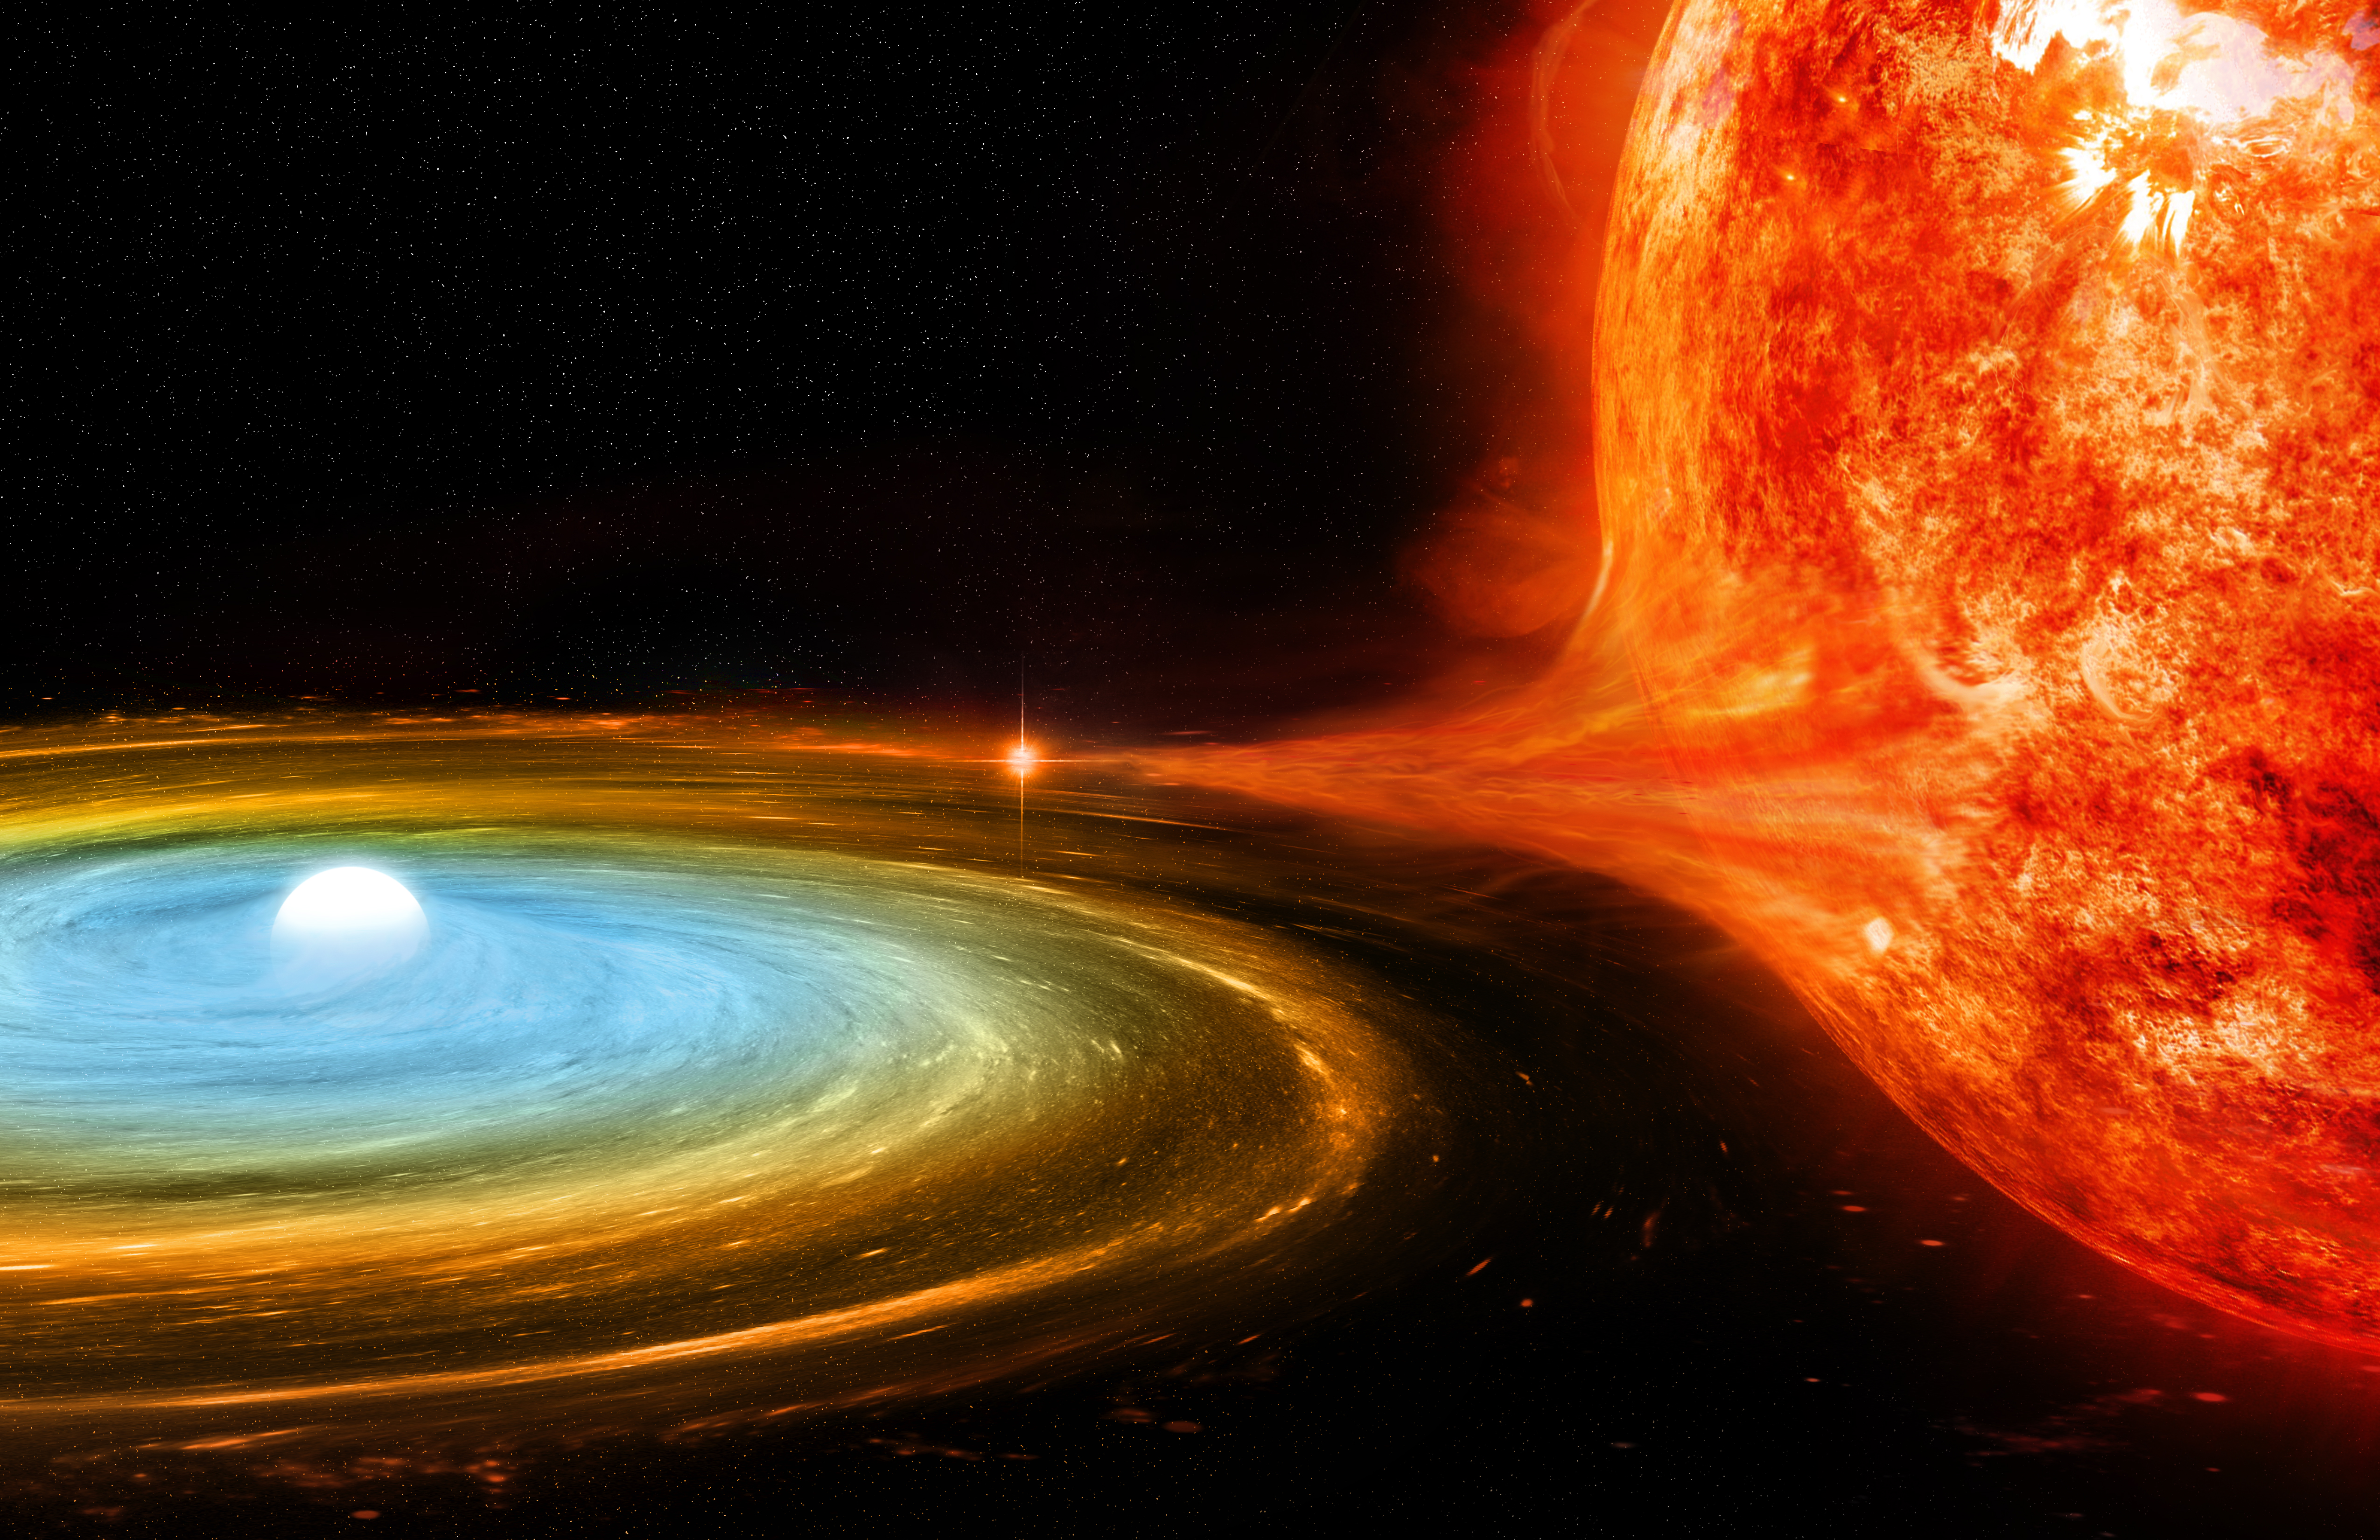
\includegraphics[width=0.88\linewidth,height=0.48\textheight,keepaspectratio]{../figs/source/en/fig-05-01.jpg}

% DOCX paragraph 479
\caption{\emph{Artistic impression of the accretion of matter in in Sco X-1. The neutron
star strips matter from its companion, which is larger in size but less massive. The
matter stolen in this way forms an accretion disc that slowly pours matter onto the
neutron star. © NASA/CXC/M. Weiss.}}\label{fig:05-01}
\end{figure}

% DOCX paragraph 481
However, something was wrong with this otherwise very reasonable scenario. To produce
such intense radiation, it is necessary that in the transfer from one star to another,
the matter undergoes a huge gravitational jump, much larger than was reasonable to
expect based on the assumed dimensions of the two stars.

% DOCX paragraph 482
To better understand this phenomenon, try to think of a hydroelectric power plant or a
water-mill. Both structures work according to the same physical principle: the
conversion of energy\index{energy!conversion} from one form, the \emph{potential
one}\index{energy!potential (gravitational)}, to another, the \emph{kinetic one}\index{energy!kinetic}. In other
words, when the water is taken from an elevated position, its fall is exploited to do
work: to operate the turbines that produce electricity or to move the wheel that grinds
the grain and transforms it into flour. The water can fall off from hundreds of metres
or from just a few metres, which clearly has an impact on the amount of work produced.
More precisely, we are converting the \emph{gravitational potential energy} into kinetic
energy. The gravitational potential energy is the energy an object (in this case, the
water) has by virtue of being in a gravitational field and is capable of releasing if
dropped, transforming it into \emph{kinetic energy} - this is the energy an object
derives from being in motion at a given speed (a stationary object has zero kinetic
energy).

% DOCX paragraph 483
In essence, this is the same conversion thought to occur in the case of Sco
X-1\index{Scorpius X-1 (Sco X-1)}: the matter subtracted from the secondary star (which represents
the water in our example) would have acquired a certain amount of kinetic energy in the
fall towards the primary, more massive but also more compact. Finally, at the moment of
the collision between the matter and the surface, the kinetic energy would have
undergone a further process. Instead of being transformed into electrical energy, as in
the case of a hydroelectric power plant, it would have produced electromagnetic
radiation in the X-ray\index{X-ray!radiation} band.

% DOCX paragraph 484
However, as we anticipated, something was wrong with this picture. Judging by the energy
produced, the gravitational leap that the matter torn from the secondary star
experienced before falling to the surface must have been enormous, much larger than one
would have expected if the primary had been an ordinary star of 1.4 solar masses.
Returning to the example of the hydroelectric power plant, it was as if the water was
falling from a mountain almost a million times higher than one would have assumed was
driving the turbine downstream. In short, the obvious discrepancy between the
theoretical expectations and the observations indicated rather clearly that there was
something decidedly wrong with the theoretical approach and, in particular, with the
type of star that the primary could be.

% DOCX paragraph 485
A further piece of observational evidence contributed to making the scenario even more
enigmatic: the X-ray\index{X-ray!radiation} source was also highly \emph{variable}. In
essence, the brightness of Sco X-1\index{Scorpius X-1 (Sco X-1)} showed significant variations over
time, with differences of 10 or 20 per cent on timescales of minutes or even tens of
seconds, much shorter than expected for an ordinary star of 1.4 solar
masses.\textsuperscript{\hyperlink{note:05-04}{4}}

% DOCX paragraph 486
The coup de grâce in this decidedly confused and disorienting picture came with the
discovery (in 1964) of another highly luminous X source, baptized Cygnus X-1 (or simply
Cyg X-1\index{Cyg X-1}). As you can guess, it was the first source in the
X-ray\index{X-ray!radiation} band at the interior of the constellation of Cygnus, the Swan.

% DOCX paragraph 487
It was once again a binary system, but the masses in question were decidedly larger: the
primary was estimated at 40 solar masses, while the secondary at 15 (therefore, baptised
as \emph{a high--mass X-ray}\index{X-ray!radiation} \emph{binary} or
HMXB\index{HMXB (High Mass X-ray Binary)}). At any rate, the brightness in the X band of Cyg X-1 was also
very high, so much so that it was anomalous. In addition, just as for Sco
X-1\index{Scorpius X-1 (Sco X-1)}, the binary system of Cyg X-1 also had a short orbital
period\index{orbit!period} (of about 5.6 days), and this allowed astronomers to see the
emission in the optical band of the primary, a star well-known to be massive and bright,
but otherwise relatively standard.\textsuperscript{\hyperlink{note:05-03}{3}} An image of Cyg X-1 in the X-ray
band is shown in Figure \ref{fig:05-02} and allows us to appreciate how difficult it is to have a
well-resolved image in the X-ray band!

% DOCX paragraph 488
Once again, however, what made Cyg X-1\index{Cyg X-1} truly mysterious was its
variability\index{variability}: it could drop below one second and even reach the order
of a few milliseconds. As we have seen, such a short time of variability implied very
small dimensions, well below 300 kilometres of radius. In those years, no known model
could explain how such a small star could produce such an emission in the X
band.\textsuperscript{\hyperlink{note:05-04}{4}}

% DOCX paragraph 491
\begin{figure}[htbp]
\centering
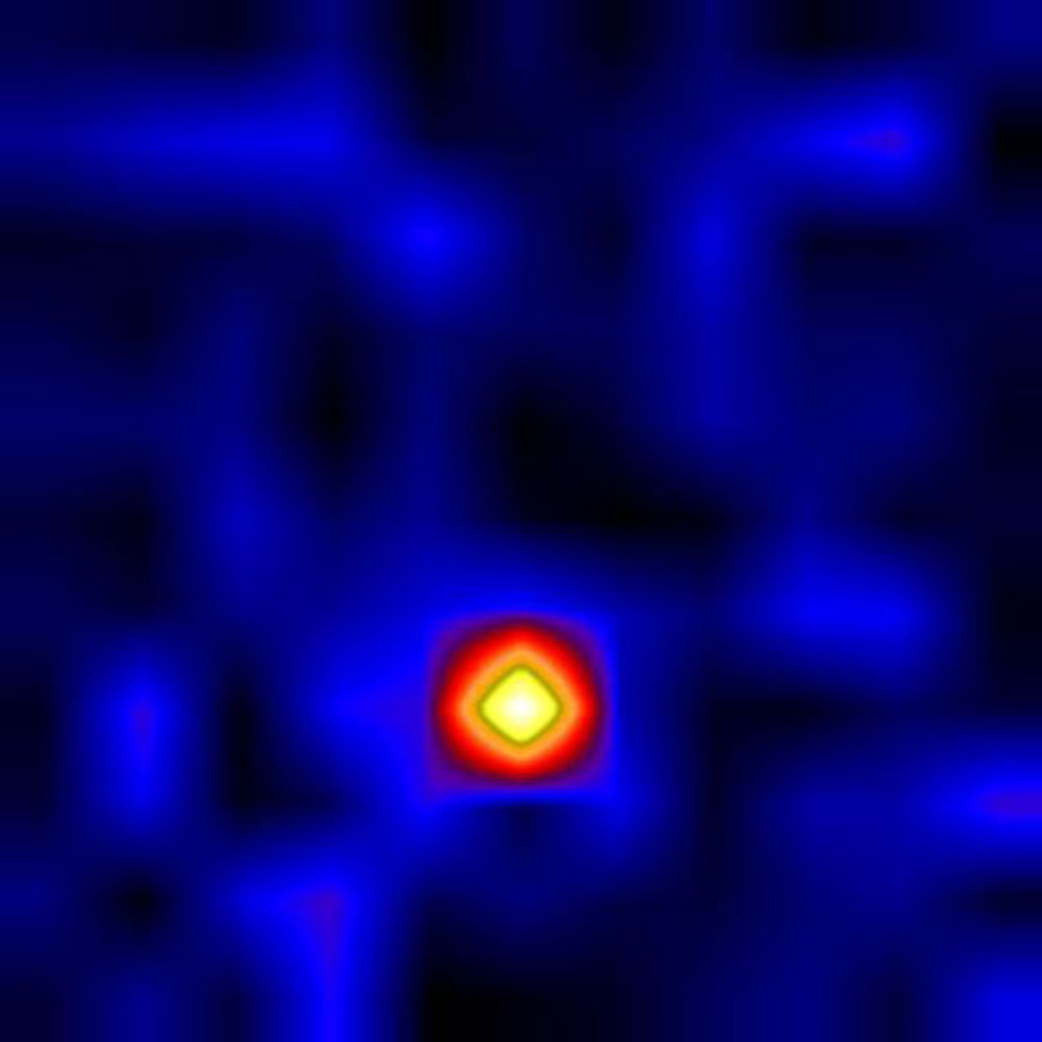
\includegraphics[width=0.88\linewidth,height=0.48\textheight,keepaspectratio]{../figs/pdf/en/fig-05-02.pdf}

% DOCX paragraph 493
\caption{Image in the \emph{X-ray band image of Cyg X-1. The emission is linked to an
accretion disk that extracts matter from a 40-solar-mass star and dumps it onto a
15-solar-masses black hole. © NASA/Marshall Space Flight Center.}}\label{fig:05-02}
\end{figure}

% DOCX paragraph 495
In short, the astronomers of the early 1960s were faced with a difficult puzzle to
solve. Observations of Sco X-1\index{Scorpius X-1 (Sco X-1)} and Cyg X-1\index{Cyg X-1}
demolished many of the certainties that nuclear astrophysics had taken about thirty
years to build. There was no doubt: the observations revealed sources of very small size
(and very little on any ``astronomical scale'') and, at the same time, extremely massive
(or having a very large mass), which produced enormous quantities of high-energy
radiation (particularly in the X band); stellar astrophysics could not explain their
nature and nuclear physics did not know any mechanism capable of shedding light on their
enormous efficiency in energy\index{energy!production efficiency} production. At the same time, however,
Sco X-1\index{Scorpius X-1 (Sco X-1)} and Cyg X-1 also represented an incredible opportunity ---
there is nothing more interesting for a scientist than discovering something apparently
inexplicable!

% DOCX paragraph 496
It soon became apparent that there was no solution to the puzzle of the two sources
unless one considered the bizarre theory of gravity proposed almost fifty years earlier
by the German physicist Albert Einstein. A theory predicting the existence of extremely
small objects capable of generating a high spacetime curvature.

% DOCX paragraph 497
In the rest of this chapter, we will learn what we know today about that wonder of
nature that is responsible for the emission of Sco X-1\index{Scorpius X-1 (Sco X-1)}.

% DOCX paragraph 500
\section{What Remains Of A Massive Star}\label{sec:05-remnant}

% DOCX paragraph 502
As happens almost systematically in astrophysics, the flourishing of a myriad of
theories and scenarios attempting to explain the observations of Sco
X-1\index{Scorpius X-1 (Sco X-1)} and Cyg X-1\index{Cyg X-1} soon followed. Most of these
hypotheses turned out to be far from reality, even though each was physically correct. A
rather common phenomenon in a scientific field such as astrophysics, in which we are
called upon to deduce physical functioning mechanisms through simple observations
without being able to create an experimental apparatus to test this or that hypothesis.
We will return to this topic at the end of Chapter 6.

% DOCX paragraph 503
The first to propose the model now believed to correctly explain the phenomena related
to Sco X-1\index{Scorpius X-1 (Sco X-1)} was the Soviet astrophysicist Iosif
Shklovsky\index{Shklovsky, Iosif} who (in February 1967) concluded that all previous
assumptions were unsatisfactory; each had aspects that appeared unrealistic or
insufficient to account for the observations. However, he was convinced that there was a
fairly simple approach to explain the phenomenology of Sco X-1\index{Scorpius X-1 (Sco X-1)}: his
model required the formation of an accretion\index{accretion disc} disc which, starting
from the secondary star, caused matter to fall onto an extremely compact object, i.e., a
\emph{neutron star}. \index{neutron star}\textsuperscript{\hyperlink{note:05-05}{5}}

% DOCX paragraph 504
What has always surprised me about the --- correct --- hypothesis put forward by
Shklovsky is that, at that time, no one had ever observed a neutron star! Since the
1930s, after the discovery of the neutron, the existence of a stellar object composed
only of those electrically neutral elementary particles was believed to be theoretically
possible, but that was all. Walter Baade\index{Baade, Walter} and Fritz
Zwicky\index{Zwicky, Fritz} proposed this idea in an article that proved to be one of the
most forward-looking in astrophysics, discussing concepts such as a
supernova\index{supernova} explosion (which we will discuss shortly), a neutron star,
and the origin of cosmic rays.\textsuperscript{\hyperlink{note:05-06}{6}} The idea of a neutron star proposed by
Baade and Zwicky was certainly not part of an organically developed theory. Indeed, it
appeared literally in a footnote of the 1934 article. Yet, in 1967 that was enough to
change the understanding of Sco X-1\index{Scorpius X-1 (Sco X-1)} and put aside different,
fascinating but incorrect interpretations.

% DOCX paragraph 505
Shklovsky\textquotesingle s model provided a simple explanation for what emerged from
the observations, albeit at the cost of introducing an ``exotic ingredient'' into his
recipe. Namely, an elusive compact object whose existence and origin were plausible from
an astrophysical point of view (it was known that massive stars could explode and,
perhaps, leave a residue), but that no one had ever identified before. There remained,
therefore, a margin of uncertainty, which collapsed at the end of that same year. In
Cambridge, the British student Jocelyn Bell\index{Bell, Jocelyn} and her supervisor Antony
Hewish\index{Hewish, Antony} identified an astronomical object capable of generating a
pulsed and regular radio emission --- the first discovery of a neutron
star.\textsuperscript{\hyperlink{note:05-07}{7}}

% DOCX paragraph 506
But what is a neutron star, and how is it formed? To answer this question, we must go
back to what we saw at the beginning of the chapter when I recalled that a star produces
energy through a series of processes of thermonuclear fusion\index{thermonuclear fusion} of
elements with increasing \emph{atomic}\index{atomic!mass}
\emph{mass}.\textsuperscript{\hyperlink{note:05-08}{8}} Hydrogen fuses to helium, helium to carbon, carbon to
neon, and so on. An essential aspect for the success of this phenomenon is the
production of a certain amount of energy each time it occurs. The amount of energy
released depends on the elements involved in the fusion: as if climbing a ladder, the
released energy increases in step with their atomic mass. Thus, the transformation of
hydrogen into helium produces less energy than the next step --- that from helium to
carbon. More importantly, each of these fusions releases energy in the form of heat and,
for this reason, they are all called \emph{exothermic thermonuclear}
\emph{reactions}\index{thermonuclear reactions!exothermic}.

% DOCX paragraph 507
As is inevitable, however, this scale has an upper limit, at which point it is no longer
possible to produce energy. Iron represents this limit, particularly by its isotope with
an atomic mass of 56 (indicated as \textsuperscript{56}Fe). Consequently, the fusion of
two of its atoms requires more energy than it releases because it is necessary to supply
the system with enough energy to bring the atoms together and merge them. Fusions of
this type, which absorb energy from the outside in the form of heat, are called
\emph{endothermic thermonuclear} \emph{reactions}\index{thermonuclear reactions!endothermic}.

% DOCX paragraph 508
Not all stars in their lifetime reach the top of this ladder; indeed, most of them (that
is, those below a dozen solar masses) stop much earlier. The reason is very simple: in
order to develop, fusion reaction processes need critical temperatures and densities,
below which they are not triggered. This is because, in general, the atoms that take
part in these reactions have a positive electric charge. Therefore, it is necessary to
reach sufficiently high temperatures and densities to allow them to overcome the
repulsive push that would tend to make two atoms with the same charge move apart. On the
other hand, the greater the mass of a star, the greater the temperature and density
inside it. Thus, ``light'' stars (with small mass) burn only light elements, while
``heavy'' stars (with large mass) can burn both light and heavy elements --- that is to
say, atoms with a large number of protons and neutrons, such as neon and silicon. In
particular, stars of the order of 20 or 30 solar masses are massive enough to reach
internal temperatures sufficient to trigger reactions involving heavier elements and,
therefore, can climb the ladder up to iron.

% DOCX paragraph 509
Since temperature and density increase as we go down towards the centre of the star, the
heavier elements are produced in the innermost regions of the star. Conversely, the
lighter ones form in the outermost areas. Over its lifetime, a massive star develops a
structure similar to an onion: the outer layers are rich in light elements, while the
innermost ones are rich in heavy elements. If the star is massive enough, its core will
be composed of iron\index{iron} produced by fusing the heavier elements, such as
neon, oxygen, and silicon.

% DOCX paragraph 510
When all the fuel that can be turned into iron runs out, the star is at a fundamental
turning point because the fusion into heavier elements would absorb energy rather than
produce it. From then on, nothing will ever be the same. As you can imagine, the
impossibility of generating new energy compromises the balance preserved up to that
moment. For millions of years, it was precisely the nuclear fusion processes that
released the energy necessary to resist the force of gravity, which otherwise would make
the star implode.

% DOCX paragraph 511
At this point, it may help us to understand what happens if we resort once again to an
analogy. Imagine a star to be like a hot air balloon, beautifully inflated with hot air
thanks to the jet of a powerful burner. From a physical point of view, the balloon
remains stretched because the pressure inside it is higher than that outside. The
release of energy that occurs when the burner combusts its fuel is the source of such
pressure. In a star, the pressure is instead produced thanks to the energy released
through nuclear reactions. When the internal pressure\index{pressure!internal} is no longer
available because the burner has run out of fuel, overwhelmed by external
pressure\index{pressure!external} and gravity, the balloon will simply deflate. The star, on
the other hand, once it has run out of fuel and cannot produce more iron, is forced to
implode under its own \emph{gravitational weight}, collapsing towards the centre.

% DOCX paragraph 512
When this occurs in a star of 20 or 30 solar masses, its core is composed entirely of
iron\index{iron} and has a radius of about 10,000 kilometres. Unable to bear its
own weight and deprived of the support of pressure, the iron core\index{iron!core}
contracts quickly, free-falling towards the centre (just like a hot air balloon would).
During this phase, the matter at the stellar core is further compressed, reaching
extreme temperatures and, above all, densities. The implosion continues until the
density in the stellar core becomes such that it ``packs'' the atoms into a very small
volume, squashing them against each other. A new, incredible pressure develops at this
point, the origin of which is not thermodynamic (i.e., linked to the fact that the
temperature must increase if the density increases) but instead quantum mechanical. The
atoms present in the free-falling iron core are compressed so much that the rules of
quantum mechanics\index{quantum mechanics} (according to which, particles such as neutrons
cannot be too close to each other) give rise to the so-called
\emph{degeneracy}\index{degeneracy!pressure} \emph{pressure}, which suddenly opposes the
contraction.\textsuperscript{\hyperlink{note:05-09}{9}}

% DOCX paragraph 513
This new and enormous pressure is able to stop the gravitational\index{gravitational!collapse}
collapse\index{collapse|see{gravitational collapse}} of the iron core, which has now reached a radius of only 100
kilometres and a temperature of billions of kelvin. It is not possible to contract
beyond that incandescent core, whose matter is the densest and most rigid we know. In
the meantime, however, the rest of the star continues to fall, ``unaware'' that the
contraction of the core has stopped: only the innermost part is subject to the
degeneracy\index{degeneracy!pressure} pressure, which creates the conditions for a spectacular
shock\index{shock} wave. At a certain point, and not being able to proceed
further, the stellar mantle ``bounces'' on the surface of the iron core, generating an
enormous \emph{shock front} that travels outwards from the heart of the star at
supersonic speed. Already saturated with the gravitational potential energy gained
during the mantle\textquotesingle s fall, the shock front is further ``pushed'' out by
the energy of the neutrinos\index{neutrino} emitted copiously from the hot and dense
core. The result is both catastrophic and spectacular: the shock wave is able to cross
the entire star, sweeping away (at enormous speeds) all of the matter it encounters. In
a few tens of seconds, a star of 20 or 30 solar masses is pulverised by a huge
explosion, namely, a \emph{supernova}. Therefore, a supernova explosion is nothing more
than the phenomenon produced by the central part of a star that ``bounces'' on hitting
the hard core created by the degeneracy\index{degeneracy!pressure}
pressure\index{neutron star!supernova}\index{supernova}.

% DOCX paragraph 514
As the outer layers of the star are blown away, an enormous amount of radiation in the
visible band accompanies the explosion, which makes the process detectable even at very
large distances. If the phenomenon occurred near us (for example, within our galaxy), it
would be possible to see it with the naked eye, even in broad daylight! And
that\textquotesingle s exactly what happened in 1054, when some Chinese astronomers
recorded the presence, in the daytime sky, of a new star. We now know this was a
supernova\index{supernova} in the constellation of the Crab\index{Crab!constellation}. These
days, astronomical observations allow us to study the ``remnants'' of explosions of this
type in what astronomers refer to as \emph{nebula}\index{nebula}\emph{e}. These are
composed of the filamentous residue of all the stellar matter that the explosion has
blown away, projecting it at enormous speed, in the order of 1,500 kilometres per second
--- in astronomical volumes equal to 10 light years. For comparison, the solar system
has a size of only five light hours.

% DOCX paragraph 515
An very nice image of the Crab nebula is shown in Figure \ref{fig:05-03}, which actually reports the
superposition of two images taken with different filters so as to highlight the various
components of the emission from the Nebula. Note how this technique allows us to clearly
appreciate the presence of the numerous filaments emanating from the centre of the
nebula and are the result of the supernova explosion. These are what is left of the
exploded star! Right at the center of this nebula there is a tiny neutron star that, as
we will learn soon, is simply a condensate of extremes.

% DOCX paragraph 517
\begin{figure}[htbp]
\centering
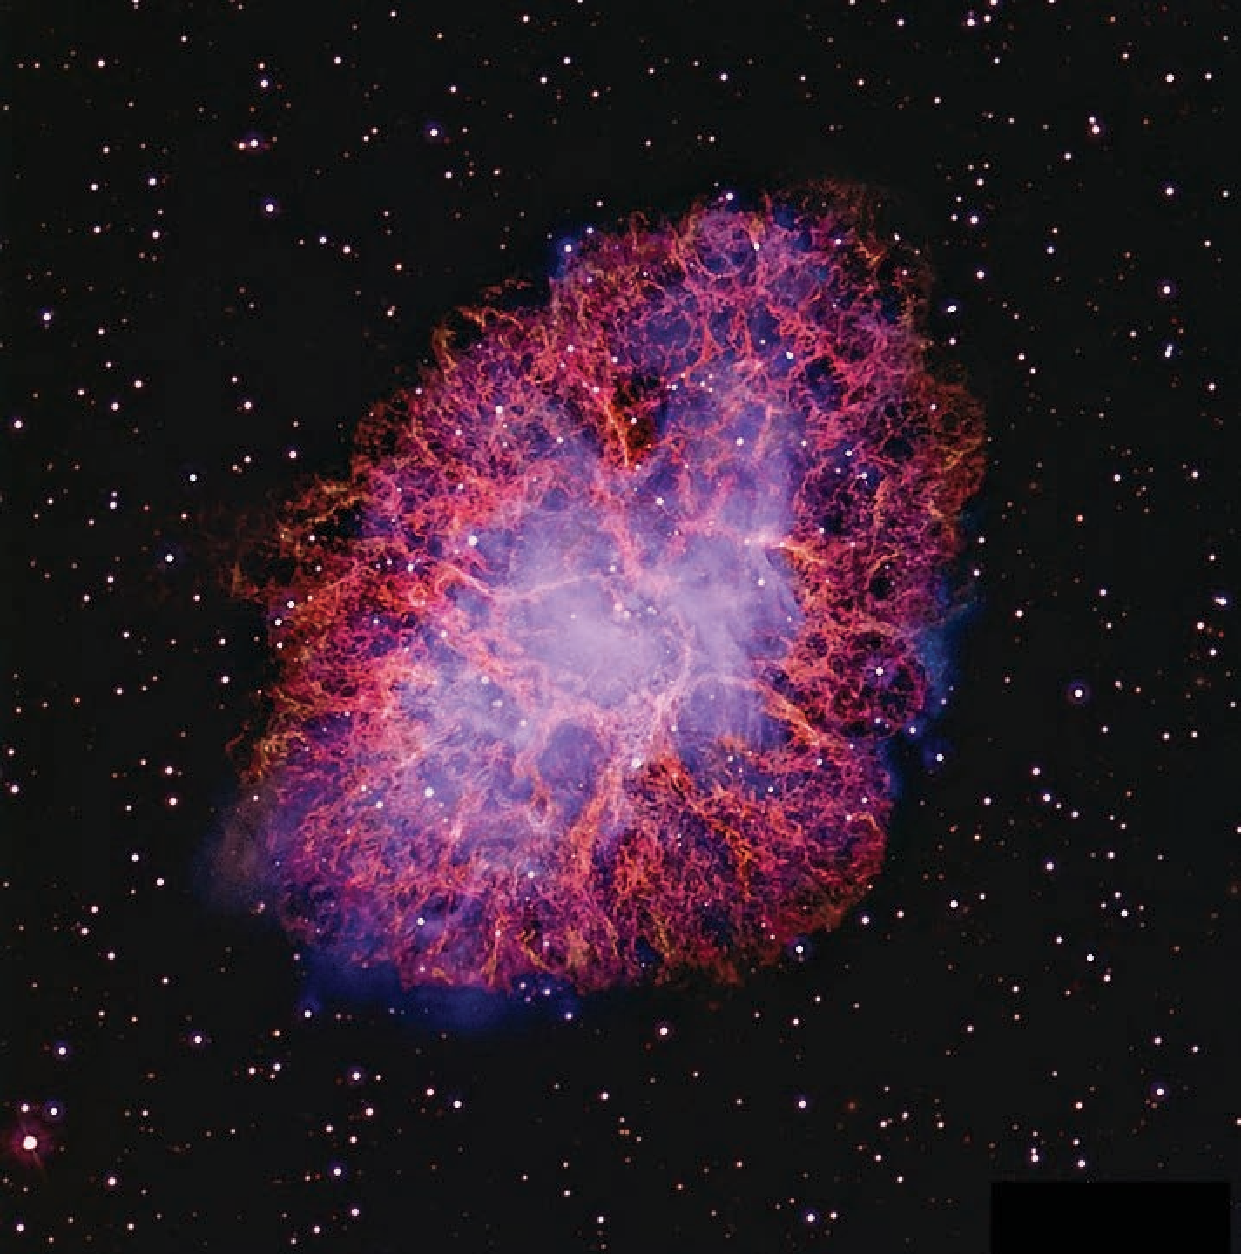
\includegraphics[width=0.88\linewidth,height=0.48\textheight,keepaspectratio]{../figs/pdf/en/fig-05-03.pdf}

% DOCX paragraph 519
\caption{\emph{Superposition of different images in the visible part of the spectrum of
the ``Crab nebula'', the remnant of the supernova explosion that took place in 1054 in
the constellation of the Cancer. © The Liverpool Telescope.}}\label{fig:05-03}
\end{figure}

% DOCX paragraph 521
Supernova explosions are very common in astrophysics, and estimates show that in our
galaxy alone, the Milky\index{Milky Way} Way, one supernova\index{supernova} can be
observed every 30 or 40 years or so. The last one (namely, SN1987A\index{SN1987A})
became visible in 1987, over 30 years ago, and astronomers are eagerly awaiting the next
one~... it will certainly be a memorable sight, which we will observe in many different
ways, as I will explain presently.

% DOCX paragraph 525
\section{A Condensate Of Extremes}\label{sec:05-extremes}

% DOCX paragraph 527
Let us go back to Sco X-1\index{Scorpius X-1 (Sco X-1)} and to what we want to discuss most in this
book: gravity. There is an object linked to one of the most extreme expressions of
physics and, indeed, of gravity whose appearance accompanies the incredible fireworks
produced by a supernova\index{supernova} explosion.

% DOCX paragraph 528
Almost invisible in the centre of a nebula\index{nebula} hides the core of the
exploded star that survived its collapse\index{gravitational!collapse}, an extremely dense and
compact celestial body whose properties cannot but arouse wonder. Personally, it has
always struck me that the final act of the bright and hectic life of a massive star (as
well as the catastrophic process that reveals its death) also marks the birth of one of
physics\textquotesingle{} most fascinating notions: a neutron star. It is an object
whose radius reaches about a dozen kilometres but which concentrates in itself a mass
much larger than that of the Sun (examples of neutron stars with two solar masses have
been observed).

% DOCX paragraph 529
Therefore, you should try to visualise a celestial body the size of the central part of
a metropolitan city like London or New York, but whose mass is enormous and whose
density is unimaginable for our sense of physical scales. In a schematic and explanatory
way, this striking contrast is shown in Figure \ref{fig:05-04}, which compares the typical
dimensions of a neutron star (with an estimated radius of between 12 and 14 kilometres)
and those of the inner part of London, bounded by its north and south circular roads.
The River Thames flows through the city west-to-east and further out the ring of the M25
orbital motorway may be seen~...

% DOCX paragraph 531
\begin{figure}[htbp]
\centering
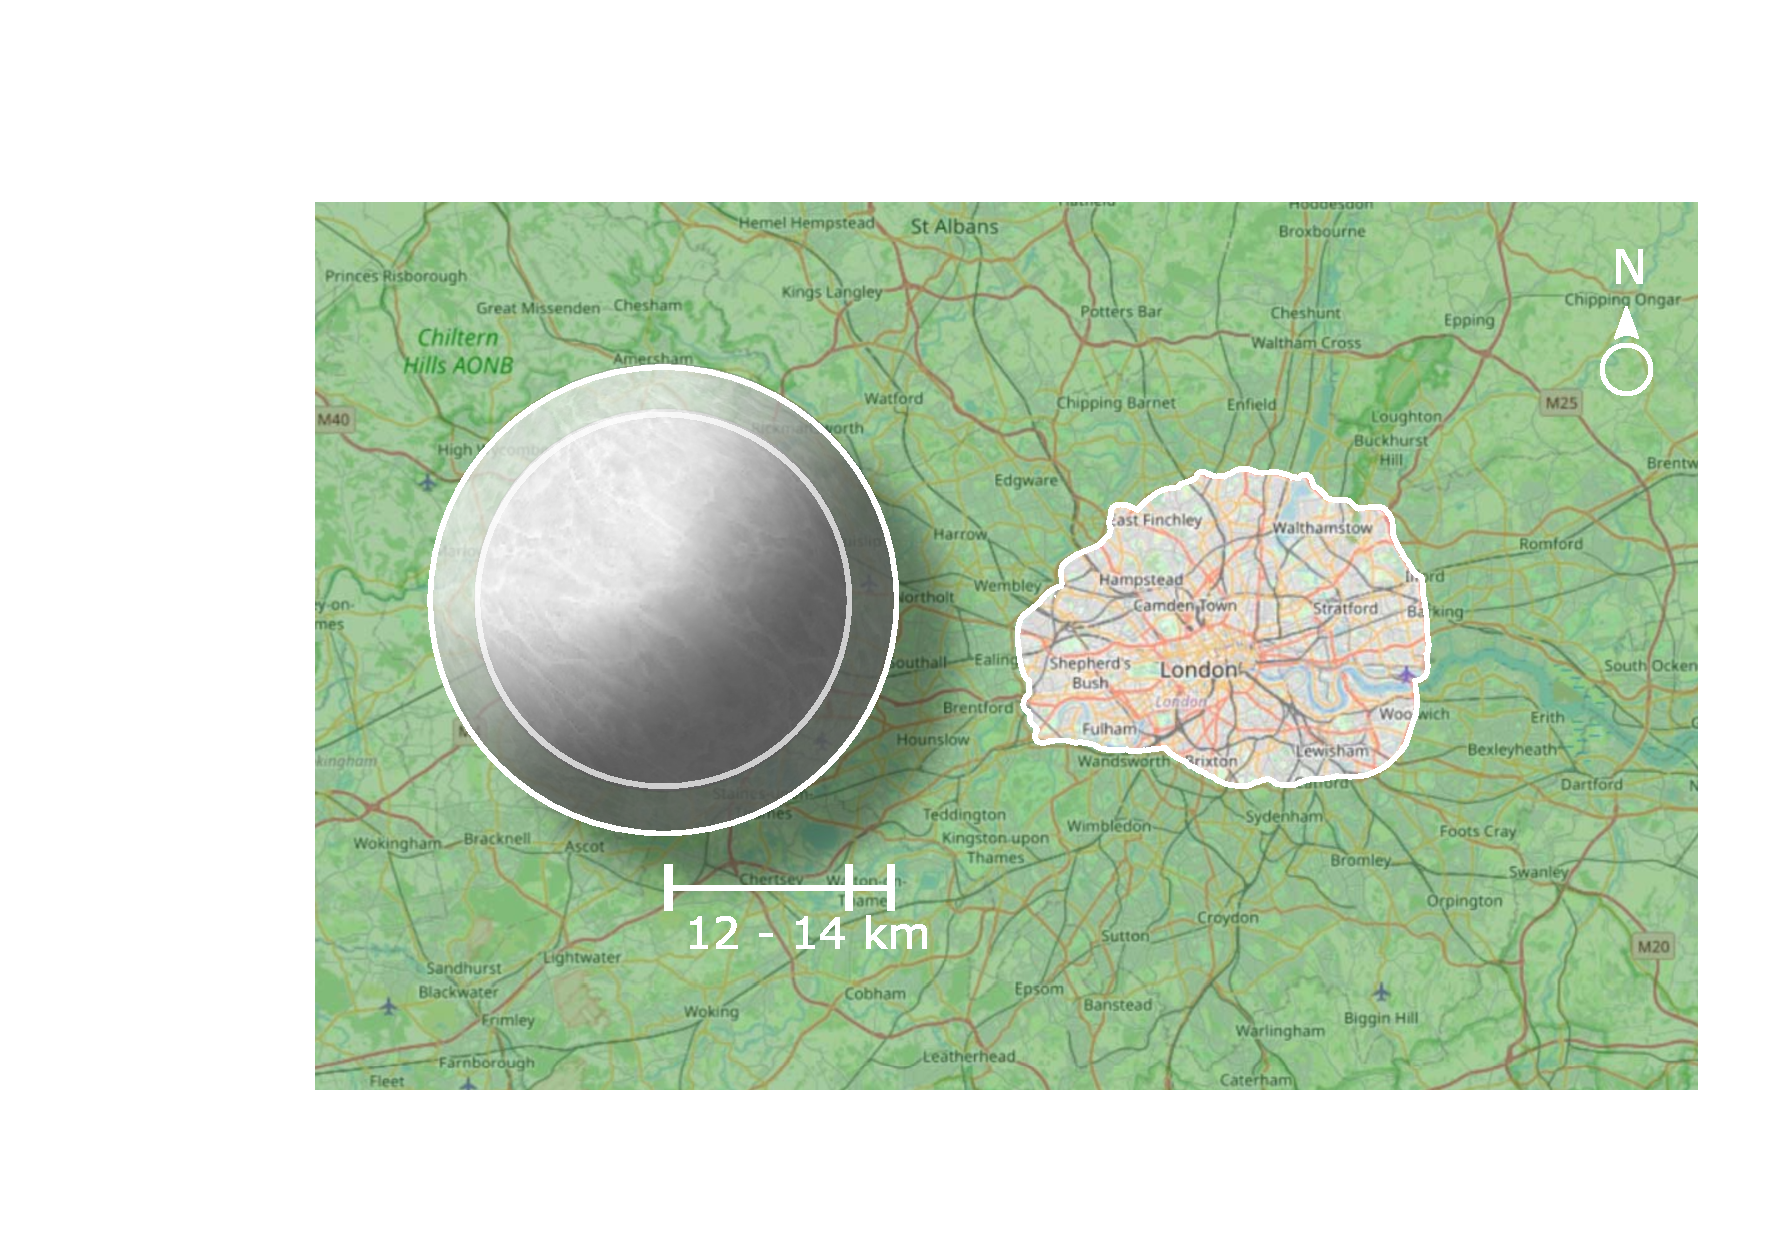
\includegraphics[width=0.88\linewidth,height=0.48\textheight,keepaspectratio,trim=149bp 72bp 41bp 96bp,clip]{../figs/pdf/en/fig-05-04.pdf}

% DOCX paragraph 533
\caption{\emph{The illustration compares the typical dimensions of a neutron star and
those of the inner part of London, bounded by its north and south circular roads. © L.
Weih / LR /map © OpenStreetMap contributors (CC-BY-SA 2.0)/ R. K. Lazenby.}}\label{fig:05-04}
\end{figure}

% DOCX paragraph 535
We have stressed several times during this journey that our sense of reality and
physical scale is necessarily determined by what we experience on this planet.
Therefore, it is difficult for us to even imagine the physical conditions that are
associated with a typical neutron star. But we can still try, starting with its density
(that is, how much matter you concentrate in a given volume). If we want to refer to a
density we are all familiar with; we could consider water: one gram per cubic
centimetre, or 1 g/cm\textsuperscript{3}. The average density of rocks is rather
similar: 2.6 g/cm\textsuperscript{3}, therefore a couple of times larger than that of
water. Well, the average density of a neutron star\index{neutron star!density} is about
10\textsuperscript{14} g/cm\textsuperscript{3}, while at its centre, it can even reach
10\textsuperscript{15} g/cm\textsuperscript{3}. In other words, we are talking about
densities that are a million billion times that of water. If you want an even more
direct comparison, try to imagine a single cubic centimetre of material coming from a
neutron star --- that is to say, as much as a sugar cube --- containing a mass equal to
the entire Alpine chain, from the Ligurian to the Friulian Alps. Warning: I am not
referring to the weight here --- although the analogy would still be correct --- but to
the number of atoms (actually protons, neutrons, and electrons) contained in our neutron
star cube. If we counted them one by one, we would discover that their number is
comparable with that of the atoms of the mountain range!

% DOCX paragraph 536
Clearly, these are densities unimaginable for us, reached when all the elementary
particles are compressed against each other, and the wave functions that describe them
are almost overlapping.\textsuperscript{\hyperlink{note:05-10}{10}} To better understand this concept, try to
think of an atom in normal conditions (those present in the matter that makes up you and
me) as a cotton candy ball, made mostly of air and strands of sugar far from each other.
In this analogy, the cotton candy represents the \emph{electronic cloud}, namely the
volume occupied by electrons\index{electron!cloud} (or rather, by their wave functions) in
their whirling rotations around the nucleus. There is something very dense and heavy at
the centre of the cotton candy, similar to one of those pellets used for fishing: the
nucleus of the atom. To understand the relative dimensions and how an atom is
essentially ``empty'', picture the cotton candy cloud is about 100,000 times larger than
the nucleus, a tiny dot but much ``heavier'' than all the rest. So, starting from this
image, we can imagine, in the atoms composing a neutron star, the virtual wiping out of
the cotton candy clouds (i.e., the electronic clouds) and only the tiny dots remaining
at their centre. In addition, these dots are packed on top of each other, at densities
more extreme than in a can of sardines. The electrons are still present in this huge
clump of nuclei but are forced to move in very small spaces and cannot create the soft
clouds that they would under normal conditions.

% DOCX paragraph 537
It would be nice (and very interesting) to reproduce these physical conditions of
extreme density in a laboratory experiment to understand, through direct measurements,
how it is possible to compress up to that point the wave functions that describe the
elementary particles at the centre of the atomic nucleus. Unfortunately, as we will see
better later, this is not possible: the densities that we are able to reproduce in the
laboratory --- even by colliding heavy nuclei with each other, launched at speeds close
to that of light inside the most powerful accelerators --- are much lower than those
that nature manages to reach in a neutron star. This creates enormous uncertainties in
our understanding of nuclear physics, the structure and composition of neutron stars. At
the same time, however, it leaves us with an equally disproportionate desire to study
and discover in order to find out how neutron stars create such physical conditions!

% DOCX paragraph 538
An unimaginable density is just one of the almost science-fiction aspects that
characterise neutron stars. Another one that amazes me every time is their ability to
rotate at very high frequencies. Indeed, we now know that some of them rotate around
their axis at a frequency of almost 700 Hz, meaning that they make 700 revolutions in
one second. If you can, try to visualise an object with a radius of a dozen kilometres
spinning around 700 times per second. For comparison, the spin of an average washing
machine reaches about 720 revolutions per minute: this means that it has a frequency of
12 Hz, i.e., it performs 12 revolutions per second. In short, it rotates roughly 60
times slower than an ordinary neutron star does\index{neutron star!rotation frequency}\index{neutron star!period}.
In principle, we know that neutron stars could even reach 1,400 Hz. However, for some
reason that we still do not fully understand, there seem to be mechanisms in nature that
put a kind of brake on the maximum rotation, forcing neutron stars to rotate below the
kilohertz.

% DOCX paragraph 539
Another source of wonder when thinking about neutron stars is that they are essentially
perfect spheres. We discovered this because (as we will see shortly) it is possible to
measure the roughness of their surface indirectly. It has emerged that the average value
for the roughness is below one-millionth of the radius, at least for those stars that
are not rotating very rapidly and that represent the large majority. This measure of the
roughness can be taken as a measure of how large the radius variation is from one point
to another. Suppose we translate this in terms of ``mountains''. In this case, it
appears that in almost all known neutron stars, the tallest surface roughness does not
exceed a millimetre in height and, in many cases, it is well below one-tenth of a
millimetre!

% DOCX paragraph 540
Let us try and make a comparison with the Earth, considering that Mount Everest has a
height of about nine kilometres: well, the maximum surface roughness of the
Earth\textquotesingle s surface is just over one part in a thousand (1/1,500, to be
precise). Therefore, although when seen from the Moon\index{Moon} our planet
appears to us as a very good approximation of a sphere, it is actually a hundred
thousand times less spherical than a neutron star. Neutron stars represent, in absolute
terms, the most spherical objects known to us: they far outweigh any sphere we can
produce in a high-precision laboratory.

% DOCX paragraph 541
But how do we know? Obviously, we cannot go on their surface to measure their roughness
with a ruler, yet we can still get fairly accurate estimates. However tiny, these
``mountains'' contain enormous quantities of matter and must, therefore, generate
gravitational waves\index{gravitational!waves (see gravitational waves)} (fear not, in Chapter 8, we will find out what
they are and why a mountain on a rotating star should produce them). In reality,
gravitational waves\index{gravitational waves} produced by mountains on neutron stars have not
yet been detected since they are incredibly weak. However, their mere presence would
produce a certain ``slowdown'' in the neutron star's rotation. Since such a slowdown has
never been measured, we consequently know how high, at most, such roughness can be. In
other words, if on the surface of a neutron star there were ``mountains''
\index{neutron star!mountains}of a certain height, they would cause a slowdown of a certain
magnitude; since this slowdown is not measured, it follows that the mountains (if any)
must be of smaller height.

% DOCX paragraph 542
Let us try to recap: we have an object with a diameter of about twenty kilometres, with
a mass greater than that of the entire solar system, which can rotate at the rate of 700
revolutions per second and is so spherical that its most ``conspicuous'' imperfection is
below a millimetre. I think even the most imaginative writers of science fiction would
have a hard time imagining it. Yet this is not science fiction; it is the irrefutable,
measurable, and wonderful reality \ldots{}

% DOCX paragraph 543
But it does not end here! Another aspect of neutron stars completely detached from our
common experience is their temperature. When we think of something extremely hot, we
inevitably end up visualising the interior of a volcano or the surface of the Sun. Well,
such environments are terribly ``cold'' when compared to neutron
stars\index{neutron star!temperature}. At the moment of their birth (i.e., when they are still
``proto-neutron stars'') \index{neutron star!proto-neutron star}, they reach 10\textsuperscript{12} K, i.e.,
one trillion kelvin. A temperature that exceeds that of the Sun by one billion times
(about 6,000 kelvin) and ten billion times that of volcanic magma (about 700 kelvin).
Such heat cannot be maintained for a long time and is mitigated by the production and
emission of neutrinos\index{neutrino} and antineutrinos\index{antineutrino}, which
subtract energy\index{energy!emission} from the star cooling it very effectively.

% DOCX paragraph 544
At the atomic level, neutrinos are produced in large quantities by converting protons
into neutrons, with the additional production of an electron\index{electron} to
conserve the electrical charge. This phenomenon has been called the
\emph{Urca}\index{Urca!process} \emph{process}, in ``honour'' of the Casino da
Urca\index{Urca!casino}, a casino in the homonymous neighbourhood of Rio de Janeiro. The
name was chosen by the physicists George Gamow\index{Gamow, George} and Mário
Schoenberg\index{Schoenberg, Mário}, who first investigated this process in
1941.\textsuperscript{\hyperlink{note:05-11}{11}} The reference to the casino is derived from the Urca process,
through the production of neutrinos, literally making energy ``disappear'' from the
proto-neutron star, just as the roulette table makes money disappear from the pockets of
the players.

% DOCX paragraph 545
As mentioned, the Urca process is indeed quite efficient. In a few seconds, the quantity
of neutrinos emitted from the supernova is ten times larger than the number of all the
particles (protons, neutrons, electrons~... ) present at this moment in the Sun. In the
case of the supernova SN1987A\index{SN1987A}\index{supernova}, some of these
neutrinos actually reached some detectors on Earth; in particular, twelve antineutrinos
(the antimatter counterpart of neutrinos) were identified by the Japanese experiment,
Kamiokande\index{Kamiokande}, in 1987, in two different waves and about two hours
before the supernova appeared in the visible band. It was a huge scientific success. At
the time, I was a young university student, and I was enormously fascinated: it was the
first detection of astronomical supernova neutrinos in history, with a total of 25
subatomic particles identified by experiments scattered all over the planet, and it
started the field of \emph{neutrino astronomy}. \index{neutrino!astronomy}\index{astronomy!neutrino}

% DOCX paragraph 546
Returning to the process of energy loss through the emission of neutrinos, this is so
efficient that in a matter of seconds from its birth, the neutron star is ``cooled'' to
a temperature of 10\textsuperscript{10} kelvin (i.e., one-hundredth of the initial
temperature). Within about a thousand years --- a period corresponding to the age of the
neutron star in the Crab Nebula\index{Crab!nebula}\index{nebula!Crab}\index{neutron star!Crab}
--- it reaches approximately one million kelvin (i.e., one-millionth of the starting
value). From that point onwards, the temperature of a neutron star decreases much more
slowly: at the venerable age of one million years, it still has a temperature equal to
100,000 kelvin and is, therefore, a hundred times warmer than the Sun. At any rate,
since the typical energy of the particles present in a neutron star is much higher
because of quantum-mechanical origin, neutron stars of this age are normally referred to
as ``cold''~...

% DOCX paragraph 550
\section{Revealed By A Beam Of Light}\label{sec:05-pulsars}

% DOCX paragraph 552
At this point, you may have been asking yourself the following, and the more than
legitimate, question: ``How do we know about the existence of neutron stars?''. The
answer takes us back in time to 1967, and to the radio observations to which everyone
now attributes the merit of having allowed the precise identification of these objects.
Being born in that year is a source of great pride for me, and also solves an annoying
practical problem; indeed, I never remember my age, also because it seems to change all
the time \ldots{} However, I remember very well that I came into the world in the year
of the discovery of neutron stars which, with the help of a little arithmetic, allows me
to work out how old I am.

% DOCX paragraph 553
Personal issues aside, in 1967, some observations aimed at studying very specific
objects eventually led to a discovery as important as it was unexpected (something,
however, that happens quite often in astronomy). A young PhD student, Jocelyn Bell, was
taking measurements with a rather rudimentary radio-wave detector built by her and her
supervisor, Antony Hewish\index{Hewish, Antony}. The goal was to monitor the radio emission
of objects discovered a decade earlier and known as \emph{quasars}\index{quasar}
Today we know that these are supermassive\index{black hole!supermassive} black holes located at the
centre of galaxies, which emit enormous quantities of radiation as a result of the
absorption of matter through an accretion\index{accretion disc} disc.

% DOCX paragraph 554
The emission that Bell and Hewish\index{Hewish, Antony} expected to measure was almost
constant over time since the variability\index{variability} of these sources is
extremely small. However, during the observations, the PhD student also began to record
a radio emission that varied with a very regular period: 1.33 seconds. In other words,
while looking for a constant radio signal, she found herself observing a source that
emitted radio waves\index{waves!radio} with astonishing regularity and with an
incredibly short period. As you will recall, a short period variability is necessarily
related to a small celestial object, which was in stark contrast to the characteristics
expected of quasars\index{quasar}.

% DOCX paragraph 555
After excluding a whole series of possible terrestrial sources and confirming that the
signal came from a very specific point in the sky, Bell and Hewish\index{Hewish, Antony}
formulated their own thesis: they hypothesised that it was the emission in the radio
band of an intense beam of radiation produced by an object rotating so fast it had to be
extremely compact. To tell the truth, the two scientists did not even overlook the
suggestive hypothesis that that signal was of alien origin, sent by a remote
civilisation intent on getting in touch with us. To jokingly underline that possibility,
Bell and Hewish\index{Hewish, Antony} baptised the periodic signal with the acronym
LGM--1\index{LGM–1 (Little Green Men)}, where the acronym stood for \emph{little green men}. As
bizarre as it may seem, the hypothesis of an alien civilisation trying to get in touch
with us earthlings is dusted off every time a radio source is identified that does not
fall among those known. The latest additions to the list of these ``alien signals'' are
so-called \emph{fast radio}\index{fast radio burst (FRB)} \emph{bursts} (or simply FRBs). Their
origin is still shrouded in mystery, but some interesting theories have been formulated,
and I have also put forward a hypothesis\ldots \textsuperscript{\hyperlink{note:05-12}{12}}

% DOCX paragraph 556
But let us go back to LGM--1. Since the radio emission appeared with periodic regularity
and seemed to pulsate, that type of source was given the name
\emph{pulsar}\index{pulsar}, a combination of \emph{pulsating} and
\emph{quasar}\index{quasar} (the objects it was originally intended to observe).
The discovery of that emission represented a huge turning point in our understanding of
astrophysics, nuclear, and gravitational physics. To underline its importance, in 1974,
Martin Ryle\index{Ryle, Martin} and Antony Hewish\index{Hewish, Antony} received the Nobel
Prize in Physics with the official reasoning: ``For their pioneering research in radio
astrophysics''. Hewish\index{Hewish, Antony} was awarded the prize precisely for the
discovery of pulsars, yet no recognition was extended to Jocelyn Bell, who had collected
the data from which it all started. To this day, there is still no convincing
explanation for this exclusion, although Bell has always claimed that the decision of
the Royal Swedish Academy of Sciences was correct.

% DOCX paragraph 557
At any rate, more than 50 years after that discovery, we now know that in 1967 Bell had
identified the radiation beam produced by the surface of an extremely compact star --- a
neutron star, in fact --- with an incredibly strong magnetic field. The details of the
mechanism (or mechanisms) that produce this radiation remain partly obscure. Still, the
whole scientific community has generally accepted the overall scenario: if a neutron
star has a strong enough magnetic field and is subject to a high enough rotation, it is
able to develop an electric field sufficiently powerful to tear
electron\index{electron!acceleration}s from its surface and, in particular, from the magnetic
poles. These free electrons are accelerated by the electric field and produce radiation
not only in the radio band, but also in the X and gamma bands, emitted in two thin
cones.

% DOCX paragraph 559
\begin{figure}[htbp]
\centering
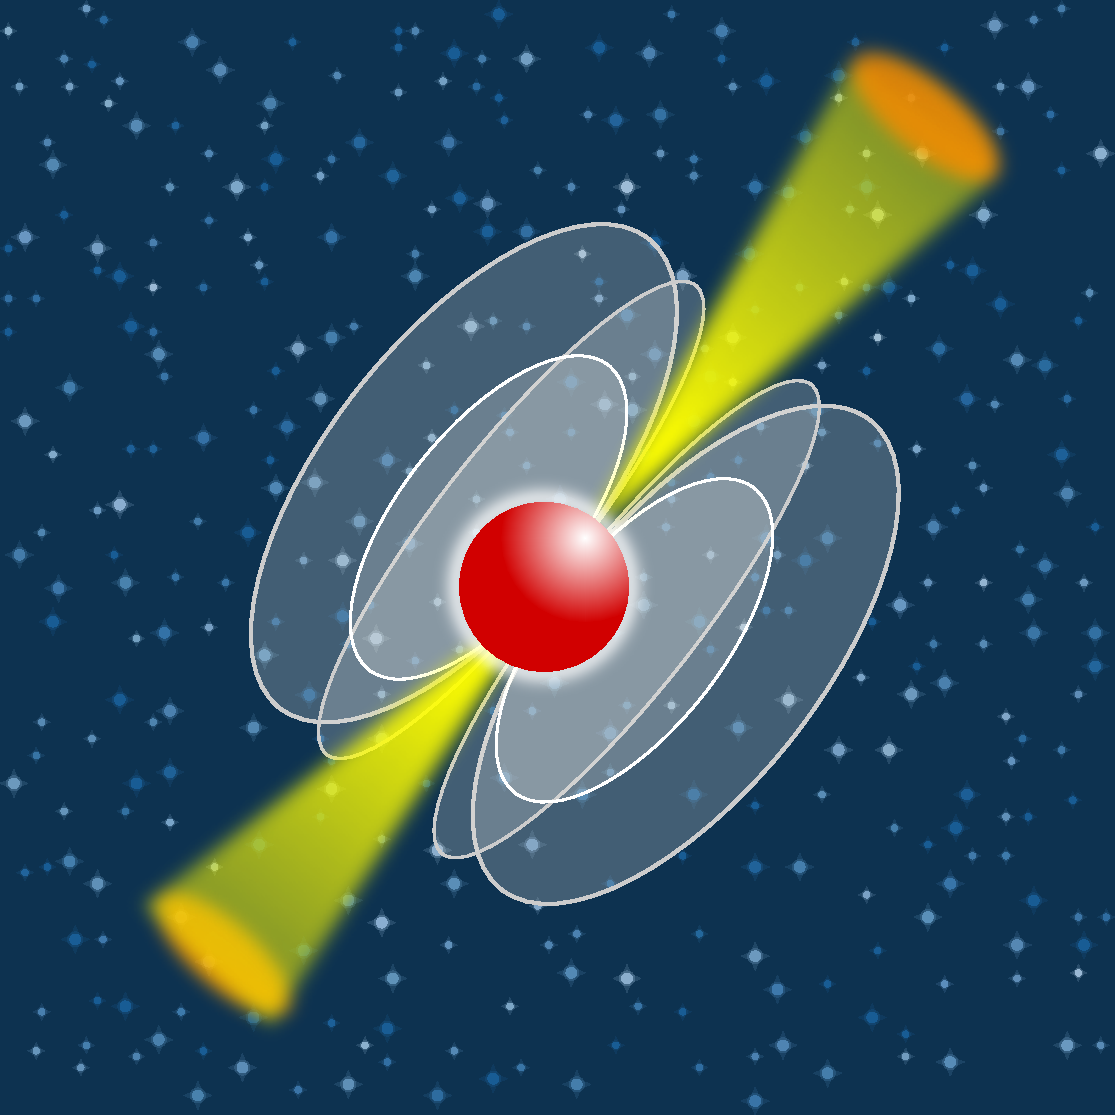
\includegraphics[width=0.88\linewidth,height=0.48\textheight,keepaspectratio]{../figs/pdf/en/fig-05-05.pdf}

% DOCX paragraph 561
\caption{\emph{In a pulsar, the rotation and strong magnetic field accelerate particles
near the polar caps, which emit collimated radiation (especially in the radio band). The
beams rotate with the star, similar to those of a lighthouse}\index{lighthouse}\emph{,
and can ``sweep'' the Earth.}}\label{fig:05-05}
\end{figure}

% DOCX paragraph 563
The operation of a pulsar is schematically represented in Figure \ref{fig:05-05}, which shows how,
in a neutron star, the combined action of a rapid rotation and a strong magnetic field
produces a thin pencil of radiation, predominantly in the radio band. The presence of a
misalignment between the axis of rotation of the star and the axis of the
dipole\index{dipole!magnetic} moment of the magnetic field causes the radiation beams to
rotate with the neutron star, periodically sweeping different regions of the sky.

% DOCX paragraph 564
Therefore, a pulsar is a rapidly rotating neutron star, emitting a beam of light in the
radio band, just as a lighthouse\index{lighthouse} emits a beam of light in the visible
band. So, when we on Earth are ``swept'' by the beam of light emitted by the neutron
star, we see a pulsed radio emission, with the pulsation period equal to that of the
rotation of the star (or half of it, if we can see both beams emitted by the poles of
the magnetic field).

% DOCX paragraph 565
An aspect that I have so far only mentioned in passing, but which is actually one of the
fundamental properties of neutron stars, is the incredible intensity of their magnetic
field: even in the most ordinary ones, it reaches values of the order of
10\textsuperscript{11} or 10\textsuperscript{12}
Gauss\index{Gauss (magnetic field)}\index{neutron star!magnetic field}\index{neutron star!pulsar (see)}. To make a comparison
with realities closer to us, the Earth's magnetic field, for instance, is about half a
Gauss, that of the Sun about one Gauss, and that of the magnetised bars (for example,
the magnets we stick on the fridge) is of the order of approximately 100 Gauss. In
short, the magnetic field of a normal neutron star is a thousand billion times more
intense than that which confronts us daily on our planet. But there are neutron stars
whose magnetic field is even more intense and can reach enormous values:
10\textsuperscript{14} or 10\textsuperscript{15} Gauss, or up to a thousand times more
intense than that of a ``standard'' pulsar.

% DOCX paragraph 566
These neutron stars take the evocative name of
\emph{magnetars}\index{magnetar}\index{neutron star!magnetar (see)} and, very rarely, can emit such
powerful flashes in the X and radio bands that, for a few moments, they are able to
overwhelm all the other celestial objects combined. To give you an idea of the absurdly
large amount of energy\index{energy!emission} released by a magnetar when it emits radiation
explosively, we can take the case of SGR 1806--20\index{SGR 1806–20}, which recorded one
of these explosions in December 2004. Calculations show that the amount of energy
emitted by this source in just one-tenth of a second exceeded that produced by the Sun
over the last 100,000 years!

% DOCX paragraph 567
The cause of these phenomena is still unknown. However, it is hypothesised that sudden
changes in the balance of the crust of these neutron stars (comparable to portentous
earthquakes) produce massive variations in the magnetic field on the surface. In turn,
this releases enormous amounts of magnetic energy\index{energy!magnetic }, which is converted
into X-ray\index{X-ray!radiation} or gamma ray radiation. The process itself is not all that
unusual, and it is observed regularly in the Sun, where it gives life to real magnetic
explosions, also called \emph{solar flares}\index{Sun!flare}.

% DOCX paragraph 568
One may well ask: ``How are such intense magnetic fields produced?''. In fact, the
origin of the enormous magnetic field of pulsar\index{pulsar!magnetic field}s and
magnetars\index{magnetar} is still the subject of intense research and debate today.
One plausible explanation --- though not the only one --- is that it is a ``fossil''
magnetic field, that is, inherited from the original star before it collapsed. In this
case, the process that comes into play is the \emph{conservation of the magnetic field
flux} (or \emph{flux-freezing}\index{flux-freezing}) during the gravitational
collapse\index{gravitational!collapse} that gives rise to the neutron star. The product between the
section of the star itself (which is proportional to the square of its radius) and the
intensity of the magnetic field should always remain the same. During the
collapse\index{gravitational!collapse}, the original star goes from a radius of more than one
million kilometres to one of only ten, so that the mere reduction of the section is
sufficient to provide an amplification factor of
(100,000)\textsuperscript{2}=10,000,000,000 times.

% DOCX paragraph 569
To understand what is happening, imagine taking a magnet, like many of us have on the
refrigerator at home, and compressing it with a hydraulic press to halve its radius: in
this way, its magnetic field will increase by a factor of four, that is
2\textsuperscript{2}. The same also happens in a collapsing star. The big difference is
that it can start from a very weak magnetic field and develop an extremely large one due
to the enormous reduction in radius caused by the collapse.

% DOCX paragraph 570
Alongside the hypothesis of the fossil origin, there is also another, namely, that the
incredible magnetic field is generated after the collapse when the neutron star is still
an extremely hot and fluid\index{fluid} object, subject to large oscillations and
looking for a new balance. Under these extreme conditions, complex phenomena of
turbulence and magnetic dynamo inside the proto neutron star\index{neutron star!magnetic field} can
amplify its magnetic field up to the values measured with the radio observations. The
latter scenario, the details of which are still difficult to reproduce through
simulations and theoretical estimates, could explain the exceptional magnetic fields
observed in magnetars\index{magnetar}.

% DOCX paragraph 571
To complete the list of the wonderful properties (in the sense that they cannot arouse
in us anything but a sense of pure wonder about neutron stars), I would like to show you
one more: they are incredibly accurate clocks. To understand how this is possible, we
must remember that, by virtue of the high rotation and the ability to emit a pencil of
light in an exquisitely periodic manner, pulsars represent the astronomical objects
measured with the greatest accuracy: the radio astronomy of pulsars is, in fact, a very
high-precision science.

% DOCX paragraph 572
To have at your disposal a signal that repeats regularly and with high frequency allows
you to collect, over the years, an enormous amount of data with precise statistical
properties. In this way, it is possible to reduce the systematic errors that usually
plague measurements and to obtain excellent accuracy. That is why the period of some
pulsar\index{pulsar!period}s is known with an accuracy of 10\textsuperscript{-15}, that is
one part in a million billion (or, in other words, with such precision that it can be
expressed with a number of which we know 15 digits exactly!). For example, this is the
case with the fastest rotating pulsar known to us, namely PSR
J0437--4715\index{PSR J0437–4715}: its period is known to be equal to 0.005757451936712637
seconds.

% DOCX paragraph 573
To get an idea of how accurate this measurement is, imagine the precision needed to
identify, one by one, all the cells present in a human being, which are approximately
30,000 billion (or approximately 3×10\textsuperscript{13}). Well, the period of PSR
J0437--4715\index{PSR J0437–4715} is known with an accuracy that is a hundred times higher!
If we had achieved this precision in biology, we would be able to ``clone'' a human
being simply by putting together the 30,000 billion cells that make it up~...

% DOCX paragraph 574
The incredible precision with which we can measure the period of pulsars also tells us
that we can use them as highly accurate cosmic clocks. Now, for a watch to be defined as
``good'', it is essential it has a regular period, but it is equally important that its
period changes in a constant and predictable way. In the case of pulsars, it changes
almost imperceptibly, but it does change. So, what matters, and is lucky for us, is
precisely that it varies on a basis that is regular and easy to predict.

% DOCX paragraph 575
The reason why the pulsar's rotation period must change is rather simple to understand.
Just like a lighthouse\index{lighthouse} (which needs electricity to function) a
pulsar\index{pulsar!beam} must tap into some form of energy to emit its beam of
radiation in the radio band. This ``reserve'' is represented by their kinetic energy. To
be more precise, the rotation of a pulsar varies, and its period becomes longer and
longer because the star loses part of its rotational kinetic energy through the emission
of electromagnetic waves\index{waves!electromagnetic} in the radio band (this is called
pulsar\index{pulsar!spin down} ``spin down''). Recognising this mechanism represents a
cornerstone in our understanding of pulsars, and the idea was first suggested by the
Italian astrophysicist Franco Pacini\index{Pacini, Franco} in 1967 (once again,
\emph{annus} \emph{mirabilis}!). He showed that a pulsar\index{pulsar!energy loss} is similar
to a rotating magnetic dipole\index{dipole!magnetic}, in short, a magnetic rod with a north
pole and a south pole in rapid rotation. The rate of change of rotation is related to
the amount of energy lost.\textsuperscript{\hyperlink{note:05-13}{13}} It is as if the emission of
electromagnetic radiation works as a ``brake'' for the stellar rotation, and one can
even measure how strong this brake is through a combination of the rotation period and
its variation over time; a measurement that takes the name of
\emph{braking}\index{pulsar!braking index} \emph{index}.

% DOCX paragraph 576
However, the energy lost by the pulsar in this way is only a very small fraction of the
available kinetic energy. That is why the period of another pulsar called PSR
J1603--7202\index{PSR J1603–7202} --- which we know to be 0.0148419520154668 seconds ---
increases by just 0.0000005 seconds every million years.\textsuperscript{\hyperlink{note:05-14}{14}} In
comparison, a precision Swiss watch ``loses'' about seven seconds a day and a quartz
watch about ten a year~... by now, you will have guessed how much neutron stars
fascinate me. However, in order not to be ``biased'', I must remind you that, with
today\textquotesingle s technology, we can build atomic clocks with even greater
accuracies than those mentioned for pulsars: only 0.0000001 seconds lost every million
years, five times less than a pulsar\index{pulsar!spin down}. However, it should also be said
that it is possible to maintain this precision only over fairly short time spans, of the
order of a few hours. Conversely, pulsars can be stable for hundreds of thousands of
years. Which, in my opinion, definitely makes them superior!

% DOCX paragraph 577
I would like to conclude by anticipating a question that some of you may have
contemplated. We have, in fact, said that a pulsar emits a collimated beam of radiation
in the radio band and that to do so it requires a huge magnetic field and a sufficiently
high rotation since it is the combination of these two elements that produces the
enormous electric fields that can accelerate charged particles. However, we have just
seen that a pulsar rotates more and more slowly, even though it will take millions of
years to slow down completely. It is therefore legitimate to ask whether, at a certain
point, the rotation of a pulsar can become so slow that it is no longer able to emit
electromagnetic radiation. The answer is yes --- a pulsar can ``turn off'', that is,
slow down so much that it is no longer visible as a lighthouse\index{lighthouse}. When
this happens, the pulsar\index{pulsar!death line} is said to have crossed the \emph{death
line}. At that point, it will no longer be visible even though it will obviously
continue to rotate and have a strong magnetic field for billions of years more. Since we
only see those neutron stars showing up as ``turned-on pulsars'', we believe there are
many more than we have seen so far!

% DOCX paragraph 580
\section{A Mysterious And Fascinating Interior}\label{sec:05-interior}

% DOCX paragraph 582
Another more than legitimate question to ask oneself here is: ``But what does the
interior of a neutron star\index{neutron star!interior} look like?''.

% DOCX paragraph 583
The answer, without much ado, can be summarised as follows: fundamentally, we do not
know! In other words, we have only a vague idea --- or, rather, many but conflicting
ideas --- about what the internal structure and composition of a neutron star is. The
reason for this ``ignorance'' is quite apparent: the physical conditions inside such an
object are far from those testable and reproducible through laboratory experiments.
Thus, it is objectively difficult, from a theoretical as well as an experimental point
of view, to extrapolate from what is known at much lower densities (and with an
enormously smaller number of particles) and reach conclusions that are valid for the
density and pressure present inside a neutron star.

% DOCX paragraph 584
That said, there are aspects of their composition and internal structure that everyone
agrees on. For example, it is quite clear that a neutron star is not made only of
neutrons but also contains other particles within it (albeit in small quantities). The
most important are certainly protons and electrons, and the latter are ultimately
responsible for the production of the massive magnetic fields we have talked about.
Electrons (and other light charged particles) are, in fact, capable of producing the
enormous electric currents necessary to generate them. Furthermore, despite the
underlying uncertainty, it is quite clear that the structure of a neutron star must be
characterised by specific areas whose thicknesses are known to us with some precision.
On the other hand, the presence of layers is true also for our planet, whose physics is
much simpler and whose structure we can investigate directly.

% DOCX paragraph 585
So, let us imagine that we ``dissect'' a neutron star in order to understand its
structure, starting from the surface and moving towards the centre\index{neutron star!structure}.
The first layer we encounter consists of a sort of atmosphere (and is technically
referred to as such), a very thin skin, not more than one centimetre thick, composed of
extremely heavy atoms and with a density billions of times higher than that of our
atmosphere. However extreme, the properties of this atmosphere are quite clear, and its
physics relatively well tested, so much so that we consider it essentially as ``known''.
As paradoxical as it is, the only part of an object with a radius of a dozen kilometres
that we believe we know in detail, in terms of its properties, is no more than one
centimetre thick.

% DOCX paragraph 586
Moving towards the centre, below the atmosphere we will find what is referred to as the
\emph{crust}. A layer with a thickness of about one or two kilometres containing heavy
ions\index{ions}, ions with a large atomic mass, but also extremely high-energy
electrons, thus called \emph{relativistic electrons}\index{electron!relativistic}. It should be
noted that the term ``crust'' can be misleading, as it is an elastic and deformable
material, somewhat similar to an extremely dense plastic substance. However, part of the
matter in the crust will still have the characteristics of a lattice, i.e., it will show
a periodic and regular structure in which the ions are at precise distances, and the
electrons are free to move between the spaces left empty. This type of lattice structure
is the one usually encountered in solid objects and is responsible for their mechanical
properties.

% DOCX paragraph 587
Below the crust, in a layer that could extend for six or seven kilometres, we will
encounter the \emph{outer core}; there, the density reaches thousands or tens of
thousands of billions (in short, 10\textsuperscript{13} or 10\textsuperscript{14}) of
grams per cubic centimetre. An enormous density but not the maximum one, which we will
meet moving towards the central zone of the neutron star, its \emph{inner core}, which
is also six or seven kilometres thick.

% DOCX paragraph 588
The properties of the matter present in the inner core remain fundamentally unknown and
represent an exceptional theoretical challenge, with which nuclear physicists have now
been confronted for almost forty years. You will not be surprised to know that there is
no shortage of hypotheses in this regard, some more conservative, others decidedly less
so. Perhaps, however, the most important and fascinating question about the physical
conditions in the deepest areas of a neutron star concerns the presence of
\emph{exotic}\index{exotic!particles} \emph{particles}, such as hyperons or even free quarks.
We talked about the latter in Chapter 1: the elementary particles constituting other
particles, such as neutrons and protons. In other words, it is possible that at the
centre of the star, as a consequence of the very high density reached in its innermost
core (whose radius does not exceed a couple of kilometres), quarks are so close to each
other that they become ``free'', that is, no longer confined within a neutron or proton,
and thus form a \emph{quark}\index{quark!soup} \emph{soup}\index{neutron star!core}. This
hypothesis is particularly fascinating because we know that a soup of this kind must
have been present in the very first moments of the universe\textquotesingle s life (up
to a hundredth of a second) and is produced, even if only for very short intervals of
time, when heavy ions\index{ions} are collided at very high energies in
experiments. The idea that this soup\index{quark!soup} is instead present in a stable
manner inside the neutron stars and can be somehow revealed (perhaps through the
emission of gravitational waves) has the potential of opening up research areas
involving scientists from all over the world, myself included.

% DOCX paragraph 589
Doubts about the internal composition of neutron stars, which we have just discussed,
are generally described as an uncertainty in the so-called \emph{equation of state}. To
be precise, when physicists speak of the equation of state\index{equation of state} of a
neutron star, they are referring to the ability to understand how the pressure (and
therefore the internal composition) of such an object varies in the passage from the
surface to the centre. The uncertainty in this regard also translates into an
uncertainty --- which is particularly serious from an observational point of view ---
about the size that a neutron star can have. Until a few years ago, the estimates of the
radius of these celestial bodies ranged fairly widely: from seven kilometres, when
calculated using equations of state that predict very compact stars, and which take the
name of \emph{soft equations of state}\index{equation of state!soft}\index{neutron star!equation of state}\emph{,} to
18 kilometres of those equations of state that predict comparatively larger stars and
that take the name of \emph{stiff equations of state}\index{equation of state!stiff}\emph{.}

% DOCX paragraph 590
Fortunately, today we have a whole series of observations --- both in the
electromagnetic channel and in the gravitational-wave channel --- that give us more
precise indications regarding the radius of a neutron star of 1.4 solar masses
(generally considered as the reference mass): it is expected, in fact, that it is
between ten and 14 kilometres. At any rate, the determination of the radius of neutron
stars represents an extremely active research area, one in which I too am a part.
Moreover, new estimates are suggested every time a new instrument provides new
measurements or when the merger of a binary system of neutron stars is detected. It is,
therefore, not excluded that the estimates given above will soon become obsolete!

% DOCX paragraph 593
\section{Maximum Mass}\label{sec:05-mass}

% DOCX paragraph 595
The idea mentioned previously of a typical radius for a reference mass allows me to
introduce an aspect that I have so far left out when presenting the properties of
neutron stars, although it is the main topic of this book: the gravity produced by such
a celestial body.

% DOCX paragraph 596
Also, from this point of view, a neutron star is an object with extreme characteristics.
The gravity it generates is, in fact, at least a billion times stronger than that
present on Earth. If, absurdly, we landed on its surface, the gravity would reduce our
spaceship --- and us inside it --- to an almost two--dimensional object: we would be
spread on a reticular surface that would extend vertically for no more than a handful of
atoms. Furthermore, since the typical compactness\index{compactness!neutron star}\index{neutron star!compactness}
of a neutron star varies from \emph{M/R} = 0.17 to \emph{M/R} = 0.25, it is clear that
we are dealing with very significant curvatures to say the least, and that give rise to
very strong relativistic effects, such as time dilation\index{time dilation} or the
curvature of light trajectories.

% DOCX paragraph 597
There is, however, a particular aspect in the relationship between gravity and neutron
stars, which represents a direct consequence of the theory of general relativity: the
existence of a \emph{maximum mass}\index{neutron star!maximum mass}. To understand what this is, it is
necessary to refer to the solutions of the Einstein equations that allow us to build
models of neutron stars in equilibrium\index{equilibrium}. Basically, after choosing an
equation of state\index{equation of state} that links the pressure inside the star to the
local density of matter, it is possible to solve Einstein equations and find an
equilibrium model representing a neutron star. At that point, by varying the mass of the
star, it is possible to obtain a ``sequence'' of models, that is, the set of neutron
stars that belong to a certain equation of state. Since we do not know the correct
equation of state, we can construct numerous sequences of this type --- I have built
almost two million of them --- all of which are physically plausible.

% DOCX paragraph 598
All these sequences share a common property: the stellar radius decreases as the mass
increases. Thinking about it, this is a fairly anomalous behaviour in astrophysics: we
are used to finding objects in which a greater mass also corresponds to a greater radius
--- just think of what happens to ordinary stars or planets. However, in the extreme
conditions of density and pressure that characterise neutron stars, the opposite is
true: as the mass grows, the radius tends to decrease.

% DOCX paragraph 599
Figure \ref{fig:05-06} shows a schematic plot of the relationship between mass and radius in a
generic neutron star. The mass (expressed in solar masses) is placed on the vertical
axis, the radius (expressed in kilometres) on the horizontal axis. The solid black line
represents the set of solutions of the Einstein equations for a certain equation of
state so that every single point on the black line is a configuration in stable
equilibrium\index{equilibrium!stable}. As can be seen, the radius tends to decrease as the mass
increases, but the latter cannot grow indefinitely. The black curve has a maximum,
indicated with a dot, beyond which the line becomes dashed: this is the so-called
\emph{unstable branch}\index{unstable branch} of the equilibrium
configurations\index{equilibrium!unstable}. In other words, although it is also possible to find
solutions to the Einstein equations in the dashed part of the line, they are however
subject to a ``gravitational instability\index{instability!gravitational}'' and thus unstable. The
corresponding neutron stars would collapse under the gravitational pull.

% DOCX paragraph 600
Therefore, every equation of state\index{equation of state} has a maximum mass, with a stable
and an unstable branch\index{unstable branch} of equilibrium\index{equilibrium} solutions;
the grey band surrounding the black curve thus represents the uncertainty introduced in
determining the radius of a neutron star due to the ignorance about its internal
structure. If the equation of state was unique and known, that band would be reduced
until it coincides with the black line. Thus, it would be possible to know exactly the
radius, the structure, and the internal composition of the star once its mass has been
fixed, perhaps through observations (as exemplified by the dotted horizontal line).
Indeed, observations provide us with very accurate measurements of the mass but are not
able to reveal the radius directly.

% DOCX paragraph 603
\begin{figure}[htbp]
\centering
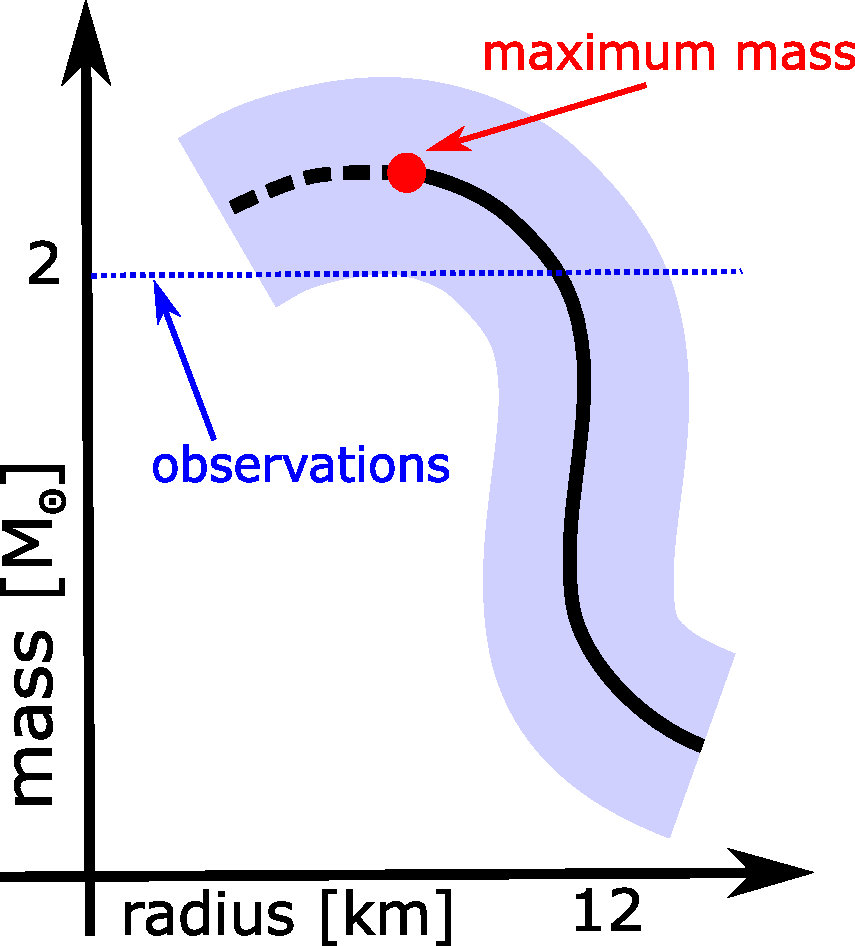
\includegraphics[width=0.88\linewidth,height=0.48\textheight,keepaspectratio]{../figs/pdf/en/fig-05-06.pdf}

% DOCX paragraph 605
\caption{\emph{Relation between mass and radius in a neutron star. The radius decreases
as the mass increases, reaching a minimum at the maximum mass. Stars with larger masses
would collapse}\index{gravitational!collapse}\emph{, so they are not possible.}}\label{fig:05-06}
\end{figure}

% DOCX paragraph 607
At this point, I would like to invite you to work out another gedanken experiment. Let
us consider a neutron star\index{neutron star!maximum mass} with a mass very close to its maximum: in
the graph, it will be almost at the top of the continuous curve, slightly to the right
and below the red dot. This star would be perfectly stable: if we perturbed it by
placing a nice hammer blow to its surface, it would respond by oscillating in a stable,
if damped, way. However, if we increased its mass even by an infinitesimal amount, for
instance, by adding a single neutron, we would take it beyond the critical point, where
it would be unstable. Its mass would exceed the maximum allowed by the equation of state
and would, therefore, be forced to do something very different from simply oscillating:
it would collapse \index{gravitational!collapse}into itself.

% DOCX paragraph 608
A maximum mass limit is not foreseen in Newton\textquotesingle s theory of gravity,
according to which it is always possible to add a little matter to a star. Likewise,
Newtonian physics does not contemplate the gravitational collapse of a neutron star with
``excessive'' mass: it is the result of the existence of additional solutions to those
of neutron stars, and we will discuss this in the next chapter. At the moment, we do not
know the value of this maximum mass. However, there is a pulsar -- PSR
J0348+0432\index{PSR J0348+0432} -- whose mass has been measured with great precision and
found to be 2.01 ± 0.04 solar masses. Since a neutron star with such a high mass exists
in nature, it follows that the maximum mass must necessarily be higher (just as shown in
Figure \ref{fig:05-06}).

% DOCX paragraph 609
Furthermore, the recent observation of the merger of a binary neutron star
system\index{neutron star!binary (see)} --- GW170817\index{GW170817} --- has provided data for new
hypotheses about this limit. Currently, many scientists --- myself included (as I argued
in an article that appeared a couple of years ago) --- think that the maximum mass
likely falls below 2.33 solar masses. In other words, the phantom maximum mass of a
neutron star is now reasonably placed between 2.0 and 2.3 solar masses. Unfortunately,
although it is a fairly narrow range, it still does not allow us to have a precise idea
of the structure and internal composition of a neutron star. However, the observations
in the years to come will provide us with many other indications, which will help us to
obtain tighter constraints on its value.

% DOCX paragraph 610
At the conclusion of this digression on the maximum mass, and as an appetiser for what
we will go on to discuss, let me anticipate that to understand what happens to a neutron
star with a mass larger than the maximum one, and thus doomed to collapse
\index{gravitational!collapse}because gravitationally \emph{unstable}\index{instability!gravitational}, we need
to understand the final state that is reached through the collapse. That is, the state
of a black hole, to which Chapter 6 is dedicated.

% DOCX paragraph 613
\section{Who's Afraid Of A Neutron Star?}\label{sec:05-danger}

% DOCX paragraph 615
Over the past fifty years, neutron stars, and pulsars in particular, have been the
subject of intense and uninterrupted observation campaigns. For this reason, we now know
of more than 2,800 pulsars, and all of the related information is freely available on
the internet through the catalogue compiled and updated by the Australian Telescope
National Facility (or, more simply, ATNF). However, the neutron stars observed so far
represent only the tip of the iceberg: in the Milky\index{Milky Way} Way alone, their
estimated population varies from two hundred thousand to one million. Most of these
pulsars are isolated, i.e., they are not associated with other stars, but there is also
a considerable fraction of them within binary systems, that is, where an ordinary star
accompanies the neutron star.

% DOCX paragraph 616
This is precisely the case with Sco X-1\index{Scorpius X-1 (Sco X-1)} --- the starting point of
this chapter --- where the neutron star strips matter from the secondary and makes it
fall onto itself in the form of an accretion\index{accretion disc} disc. When the matter
stolen from the companion falls on the neutron star, the huge gravitational leap it
experiences (remember hydroelectric power plants?) causes it to heat up, reaching
temperatures of one million kelvin, thus producing the X-ray\index{X-ray!radiation} emission
that allowed us to reveal it.

% DOCX paragraph 617
However, binary systems of this type can reach even higher temperatures! Thinking about
it, the matter deposited on the surface of the neutron star must also go somewhere. As
far as we know today, it accumulates in a layer just a few centimetres thick (let us not
forget that the gravity on the surface of a neutron star is enormous). Since the
ordinary star's outer parts are composed of light elements such as hydrogen and helium,
the transfer of matter from the ordinary star to the neutron star only deposits matter
with low atomic mass (hydrogen or helium), which is therefore highly ``combustible'' via
thermonuclear fusion\index{thermonuclear fusion}. Thus, as the stripped matter accumulates and
heats up on the surface of the neutron star, the right conditions of density and
temperature can be reached in order for a thermonuclear fusion reaction to be triggered
in that thin skin, which literally destroys the accumulated layer, causing it to lift
off the surface into a dazzling sphere of light.

% DOCX paragraph 618
This massive nuclear explosion, involving a considerable portion of the entire surface
of the neutron star\index{neutron star!X-ray burst}, releases an amount of energy equal to nearly one
billion billion atomic bombs. Furthermore, this huge release of energy occurs on a
timescale ranging from one to ten seconds. It gives life to the process that astronomers
refer to as an \emph{X-ray}\index{X-ray!radiation} \emph{burst} that characterises, in a
manner that is more or less regular, the emission of sources in low-mass
X-ray\index{X-ray!radiation} binary systems (LMXBs). Neutron stars have not only been
observed in LMXBs, they are also present in other configurations and, in particular, in
binary systems composed of two neutron stars. A special subclass of these systems is
then represented by those binary systems in which both neutron stars are also pulsars
and are called, for this reason, \emph{binary
pulsars}\index{pulsar!binary}\index{neutron star!binary pulsars}. We will return to them in Chapter 8,
when we discover that they represent extremely intense sources of gravitational waves
and very rich laboratories in which to study the properties of gravity within very
strong fields.

% DOCX paragraph 619
At this point, however, I would like to conclude this chapter with a logical question,
one that some of you may have already asked given the extreme characteristics --- in
every sense --- of neutron stars: ``Should we be afraid of these celestial objects?''.

% DOCX paragraph 620
Just like any natural phenomenon of great beauty and equal power, such as an erupting
volcano, it is also advisable to observe neutron stars from a ``safe distance''. This is
because their properties can prove to be decidedly dangerous for us fragile human
beings. However, the closest neutron star to us --- namely RX
J1856.5--3754\index{RX J1856.5–3754} --- is 500 light years away (remember that the closest
ordinary star, apart from the Sun, is only 4.24 light years away from us: Proxima
Centauri\index{Proxima Centauri}). In addition, neutron stars are not static and indeed
normally move at relatively high speeds (between 200 and 400 kilometres per second),
which they acquire at birth through the supernova explosion. The emission of
neutrinos\index{neutrino! anisotropic emission} in the first milliseconds of the
protostar\textquotesingle s life is highly \emph{anisotropic}\index{anisotropic (neutrino emission)} (that
is, it has different intensities in different directions), and this causes the protostar
to experience a ``recoil'' in a given direction, in which it will continue to wander for
the rest of its existence.

% DOCX paragraph 621
Now, if a neutron star like RX J1856.5--3754\index{RX J1856.5–3754} were to cross the solar
system, even without colliding with any of its planets (remember it is a tiny object
that, if compared to the scale of the other celestial bodies present in the solar
system, would be essentially a dot, slightly larger than an asteroid), it would create
``considerable'' gravitational disruption due to its imposing mass, certainly greater
than that of the Sun. It would break some of the orbits\index{orbit} of our
system, and if it passed close to one of the planets, for example, Jupiter (the
largest), it would simply destroy it thanks to the enormous tidal
forces\index{tidal forces} that would develop.

% DOCX paragraph 622
On the other hand, if a magnetar exploded near us, flooding us with very high-energy
radiation, this would be sufficient to erase all life on Earth within seconds. This
would be the case even for areas of the planet in the shadow of the
X-ray\index{X-ray!radiation} emission, which would instead be flooded by the radiation
reflected from other planets or the Moon\index{Moon}. In other words, I think we
can all agree that it would be advisable to avoid too close an encounter with a neutron
star, especially if it is emitting large amounts of radiation.

% DOCX paragraph 623
That said, we have very little to worry about: the magnetars\index{magnetar} within
our galaxy are known, and all very distant from us. And even if pulsar RX
J1856.5--3754\index{RX J1856.5–3754} was directed exactly towards Earth at the maximum speed
allowed by a neutron star, it still would not arrive here for six million years. So, in
essence, at least for the time being, we have nothing to fear from neutron stars and,
instead, we can enjoy the wonders they reveal to us~...
